\documentclass{article}


% if you need to pass options to natbib, use, e.g.:
\PassOptionsToPackage{numbers, compress}{natbib}
% before loading neurips_2024


% ready for submission
\usepackage[preprint]{neurips_2024}


% to compile a preprint version, e.g., for submission to arXiv, add add the
% [preprint] option:
%     \usepackage[preprint]{neurips_2024}


% to compile a camera-ready version, add the [final] option, e.g.:
%     \usepackage[final]{neurips_2024}


% to avoid loading the natbib package, add option nonatbib:
%    \usepackage[nonatbib]{neurips_2024}


\usepackage[utf8]{inputenc} % allow utf-8 input
\usepackage[T1]{fontenc}    % use 8-bit T1 fonts
\usepackage{amsthm, amsmath, amsfonts, amssymb, bm, bbm} % Math packages
\usepackage{graphicx}
\usepackage{url}            % simple URL typesetting
\usepackage{booktabs}       % professional-quality tables
\usepackage{amsfonts}       % blackboard math symbols
\usepackage{nicefrac}       % compact symbols for 1/2, etc.
\usepackage{microtype}      % microtypography
\usepackage{xcolor}         % colors
\usepackage[labelfont={small,bf},textfont={small},labelsep=space,tableposition=top]{caption}
\usepackage{subcaption}
\usepackage[ruled,linesnumbered,vlined]{algorithm2e}
\usepackage[colorlinks=true, allcolors=blue]{hyperref}
\usepackage{fixltx2e}

\usepackage{mathtools}
\usepackage{xargs}
\usepackage{soul}

\DeclareMathOperator\prox{prox}%											proximal mapping
\DeclareMathOperator*\minimize{minimize}%									minimize


\newcommand{\N}{\mathbb N}%												    naturals
\newcommand{\Z}{\mathbb Z}%												    naturals
\newcommand{\R}{\mathbb{R}}
\newcommand{\func}[3]{#1:#2\rightarrow#3}%									f: A --> B function \func{f}{A}{B}


\newcommandx\seq[3][{2=k\in\N},{3={}}]{(#1)_{#2}^{#3}}%						sequence \seq{x^k}[k=1][n]


\newtheorem{ass}{Assumption}
\newtheorem{prop}{Proposition}
\newtheorem{remark}{Remark}
\newtheorem{lem}{Lemma}


\newcounter{mysubequations}
\renewcommand{\themysubequations}{(\alph{mysubequations})}
\newcommand{\mysubnumber}{\refstepcounter{mysubequations}\themysubequations}

\newcommand{\pourya}[1]{{\color{blue}{#1}}}
\newcommand{\doublecheck}[1]{{\color{brown}{#1}}}



\newtheorem{theorem}{Theorem}
\DeclareMathOperator*{\argmin}{arg\,min}
\DeclareMathOperator*{\argmax}{arg\,max}
\DeclareMathOperator{\clamp}{clamp}
\DeclareMathOperator{\round}{round}

\title{Quantization-free Lossy Image Compression Using Integer Matrix Factorization}


% The \author macro works with any number of authors. There are two commands
% used to separate the names and addresses of multiple authors: \And and \AND.
%
% Using \And between authors leaves it to LaTeX to determine where to break the
% lines. Using \AND forces a line break at that point. So, if LaTeX puts 3 of 4
% authors names on the first line, and the last on the second line, try using
% \AND instead of \And before the third author name.


\author{%
Pooya Ashtari$^{1}$\thanks{Corresponding author. Emails:\texttt{pooya.ashtari@esat.kuleuven.be}, \texttt{pooya.ash@gmail.com}}\ \ \thanks{Equal contribution} \\
\texttt{pooya.ashtari@esat.kuleuven.be} \\
\vspace{-20pt}
\And
Pourya Behmandpoor$^{1}$\footnotemark[2] \\
\texttt{pourya.behmandpoor@kuleuven.be} \\
\vspace{-20pt}
\And
Fateme Nateghi Haredasht$^{2}$ \\
\texttt{fnateghi@stanford.edu} \\
\vspace{-20pt}
\And
Jonathan H. Chen$^{2}$ \\
\texttt{jonc101@stanford.edu} \\
\vspace{-20pt}
\And
Panagiotis Patrinos$^{1}$ \\
\texttt{panos.patrinos@esat.kuleuven.be} \\
\And
Sabine Van Huffel$^{1}$ \\
\texttt{sabine.vanhuffel@kuleuven.be} \\
\And
\vspace{-20pt} \\
\small{$^{1}$Department of Electrical Engineering (ESAT), STADIUS Center, KU Leuven, Belgium} \\
\small{$^{2}$Department of Medicine, Stanford University, Stanford, CA, USA} \\
  % examples of more authors
  % \And
  % Coauthor \\
  % Affiliation \\
  % Address \\
  % \texttt{email} \\
  % \AND
  % Coauthor \\
  % Affiliation \\
  % Address \\
  % \texttt{email} \\
  % \And
  % Coauthor \\
  % Affiliation \\
  % Address \\
  % \texttt{email} \\
  % \And
  % Coauthor \\
  % Affiliation \\
  % Address \\
  % \texttt{email} \\
}


\begin{document}


\maketitle


\begin{abstract}
Image compression is essential for efficient transmission and storage.  Widely used methods, such as JPEG, use transforms like the discrete cosine transform (DCT) that map image data into a continuous domain, which necessitates carefully designed quantization techniques. Another promising approach relies on low-rank approximation methods, such as singular value decomposition (SVD). While current methods based on this approach also require quantizers, their compression performance is unfortunately suboptimal due to their higher sensitivity to quantization errors than JPEG. Therefore, we introduce a variant of integer matrix factorization (IMF) that forms the basis for our quantization-free lossy image compression method. IMF provides a low-rank representation of the image data as a product of two smaller factor matrices with bounded integer elements, thereby eliminating the need for quantization. Moreover, the reshaped factor matrices can be treated as grayscale images, allowing any lossless image compression standard to be seamlessly integrated into the proposed IMF framework. We propose an efficient, provably convergent iterative algorithm for IMF using a block coordinate descent (BCD) scheme, where each column of a factor matrix is updated one at a time using a closed-form solution. The experiments show that our IMF method outperforms JPEG, achieving improvements of over 4 dB and 7 dB in PSNR at 0.15 bits per pixel (bpp) on the Kodak and CLIC datasets, respectively. We also assessed the ability of the methods to preserve visual semantic information by evaluating an ImageNet pre-trained classifier on compressed images. Notably, the IMF method yielded over a 20\% relative improvement in top-1 accuracy over JPEG at bit rates under 0.2 bpp.
\end{abstract}

\section{Introduction} \label{sec: introduction}



\section{Related Work} \label{sec: related work}

\paragraph{Transform-based compression.} 

\paragraph{Low-rank approximation for compression.} 

\paragraph{Integer Matrix Factorization.} 

\section{Method} \label{sec: method}


\subsection{Overall Encoding Framework} \label{sec: overall encoding framework}

\begin{figure}[t]
	\centering
	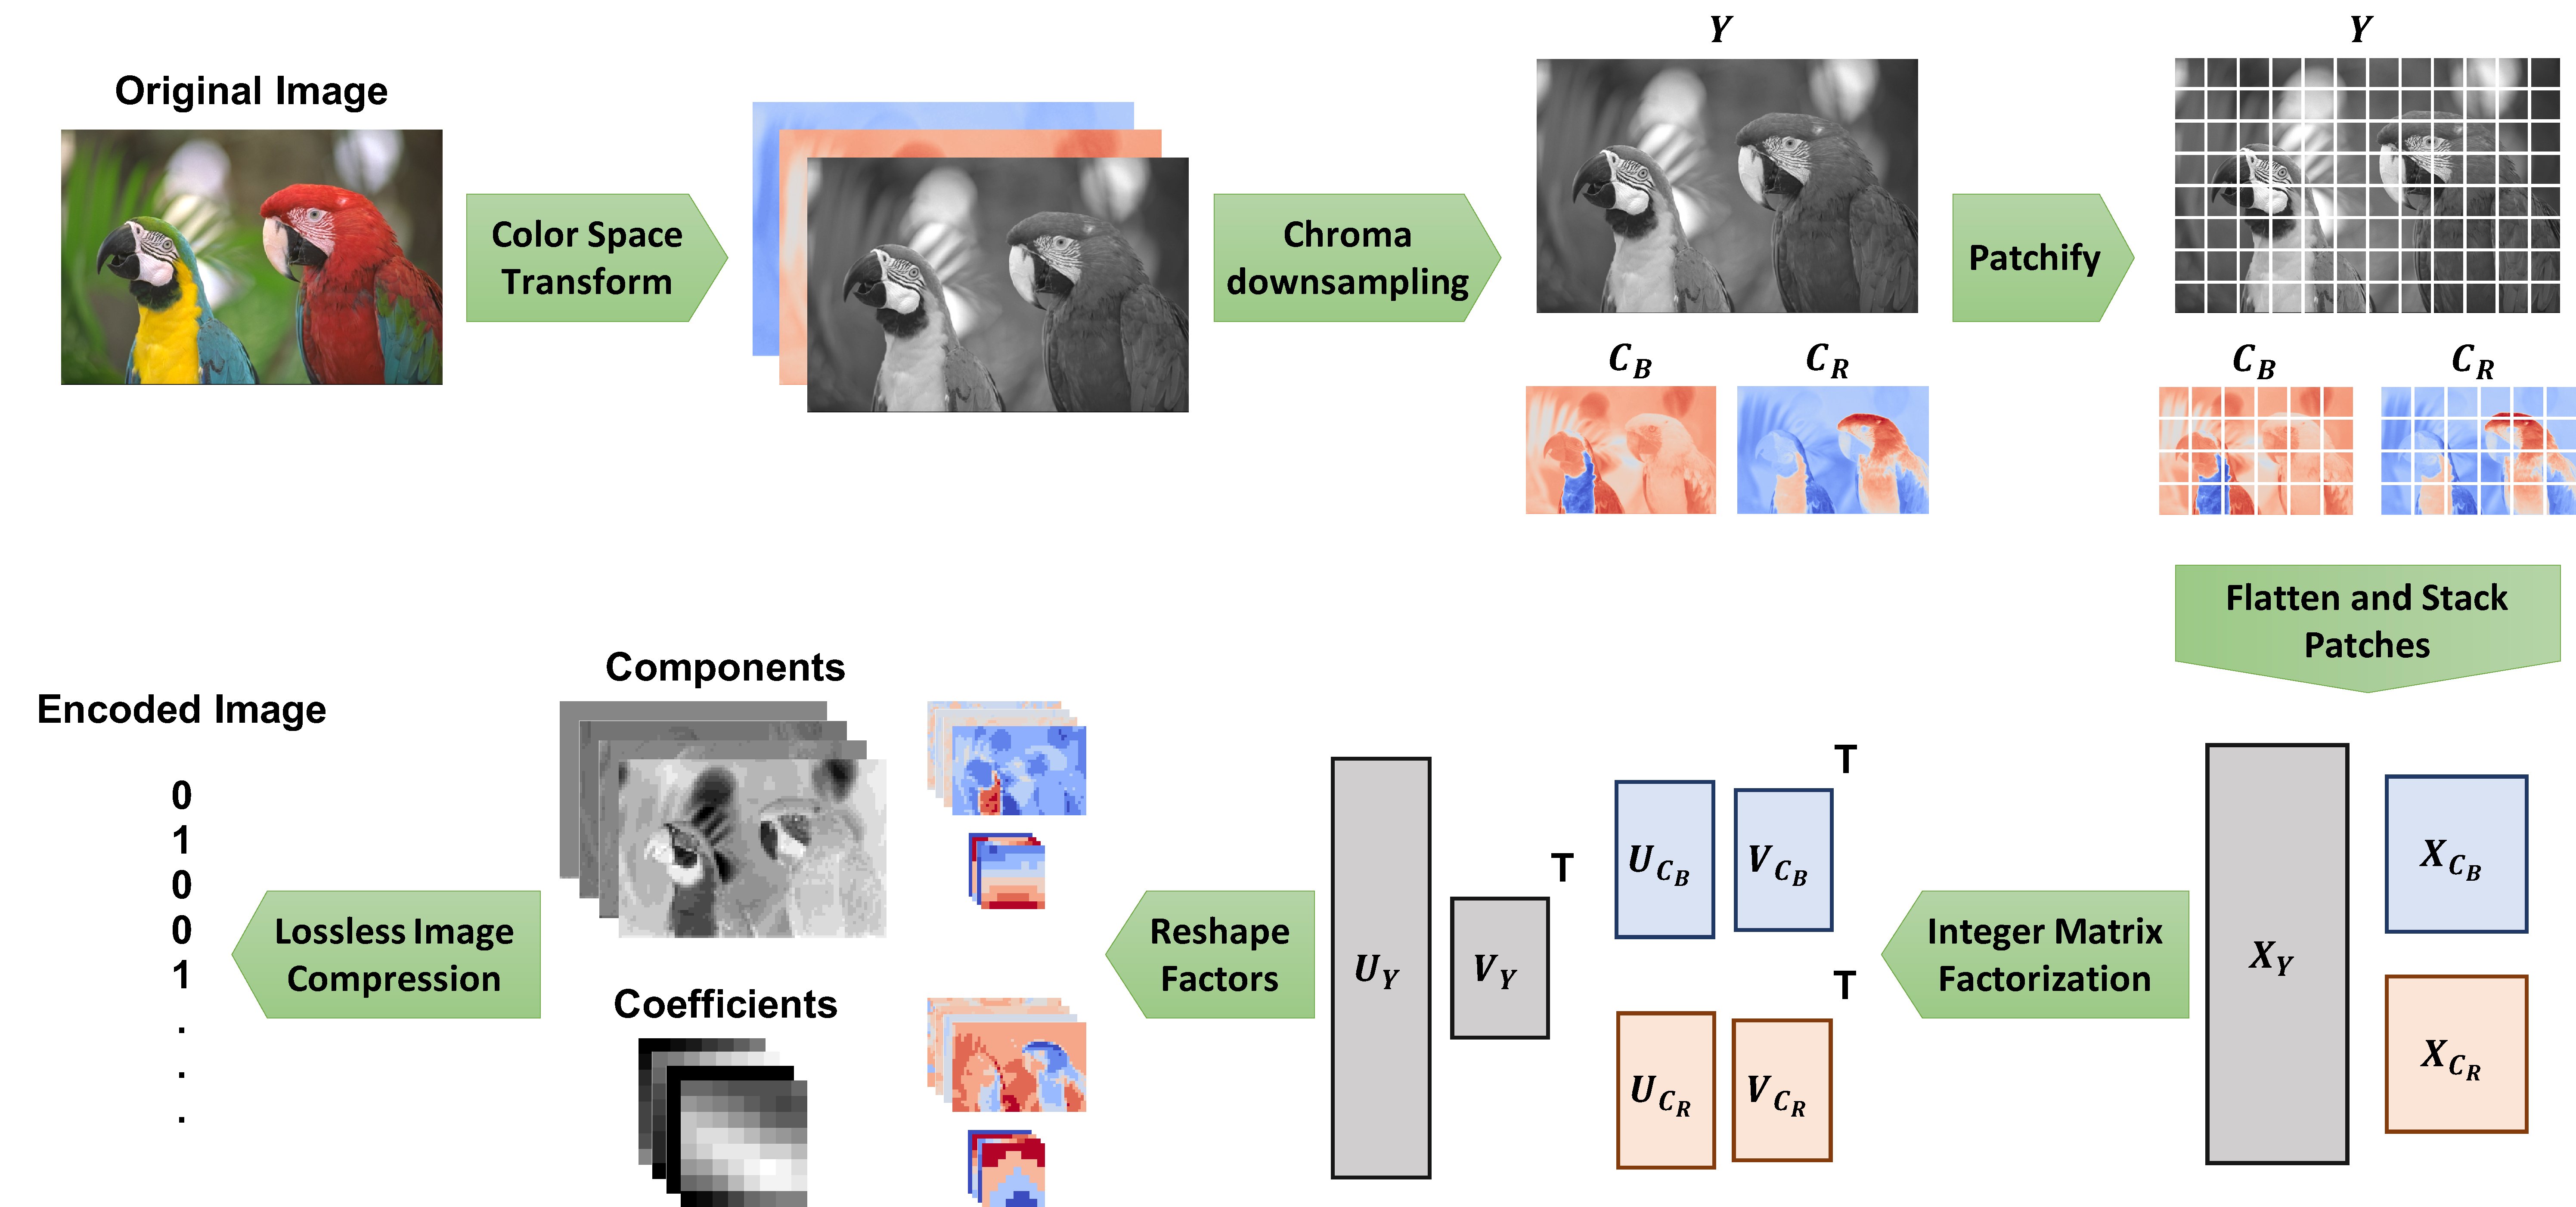
\includegraphics[width=\linewidth]{figures/imf_encoder.pdf}
	\vspace{10pt}
	\caption{An illustration of the encoder for our image compression method, based on integer matrix factorization.}
	\label{fig: imf_encoder}
\end{figure}

The proposed compression method follows a \emph{transform coding} paradigm, but it does not involve quantization. Figure \ref{fig: imf_encoder} illustrates an overview of the encoding pipeline of our method based on integer matrix factorization (IMF). The encoder accepts an RGB image with dimensions $H \times W$ and a color depth of 8 bits, represented by the tensor $\bm{\mathcal{X}} \in \{0, \ldots, 255\}^{3 \times H \times W}$. Each step of encoding is described in the following.

\paragraph{Color Space Transformation.}
Analogous to the JPEG standard, the image is initially transformed into the YC\textsubscript{B}C\textsubscript{R} color space. Let $\bm{Y} \in [0, 255]^{H \times W}$ represent the \emph{luma} component, and $\bm{C}_B, \bm{C}_R \in [0, 255]^{\frac{H}{2} \times \frac{W}{2}}$ represent the blue-difference and red-difference \emph{chroma} components, respectively. Note that as a result of this transformation, the elements of the \emph{luma} ($\bm{Y}$) and \emph{chroma} ($\bm{C}_B$, $\bm{C}_R$) matrices are not limited to integers and can take any value within the interval $[0, 255]$.

\paragraph{Chroma Downsampling.} 
After conversion to the YC\textsubscript{B}C\textsubscript{R} color space, the \emph{chroma} components $\bm{C}_B$ and $\bm{C}_R$ are downsampled using average-pooling with a kernel size of $(2, 2)$ and a stride of $(2, 2)$, similar to the process used in JPEG. This downsampling exploits the fact that the human visual system perceives far more detail in brightness information (\emph{luma}) than in color saturation (\emph{chroma}).

\paragraph{Patchification.}
After \emph{chroma} downsampling, we have three components:  the \emph{luma} component $\bm{Y} \in [0, 255]^{H \times W}$ and the \emph{chroma} components $\bm{C}_B, \bm{C}_R \in [0, 255]^{\frac{H}{2} \times \frac{W}{2}}$. Each of the matrices is split into non-overlapping $8 \times 8$ patches. If a dimension of a matrix is not divisible by 8, the matrix is first padded to the nearest size divisible by 8 using reflection of the boundary values. These patches are then flattened into row vectors and stacked vertically to form matrices $\bm{X}_{Y} \in [0, 255]^{\frac{HW}{64} \times 64}$, $\bm{X}_{C_B} \in [0, 255]^{\frac{HW}{256} \times 64}$, and $\bm{X}_{C_R} \in [0, 255]^{\frac{HW}{256} \times 64}$. Later, these matrices will be low-rank approximated using integer matrix factorization (IMF). Note that this patchification technique differs from the block splitting in JPEG, where each block is subject to discrete cosine transform (DCT) and processed independently. This patchification technique not only captures the locality and spatial dependencies of neighboring pixels but also performs better when combined with the matrix decomposition approach for image compression.

\paragraph{Low-rank approximation.} 
We now apply a low-rank approximation to the matrices $\bm{X}_{Y}$, $\bm{X}_{C_B}$, and $\bm{X}_{C_R}$, which is the core of our compression method that provides a lossy compressed representation of these matrices.  The low-rank approximation \citep{eckart1936approximation} aims to approximate a given matrix $ \bm{X} \in \mathbb{R}^{M \times N} $ by 
\begin{equation} \label{eq: lra}
	\bm{X} \approx \bm{U} \bm{V}^\mathsf{T} = \sum_{r=1}^{R} U_{:r} {V_{:r}}^\mathsf{T},
\end{equation} 
where $\bm{U} \in \mathbb{R}^{M \times R}$ and $\bm{V} \in \mathbb{R}^{N \times R}$ are \emph{factor matrices} (or simply \emph{factors}), $R \leq \min(M,N)$ represents the \emph{rank}, $U_{:r}$ and $V_{:r}$ represent the $r$-th columns of $\bm{U}$ and $\bm{V}$, respectively. We refer to $\bm{U}$ as the \emph{basis matrix} and $\bm{V}$ as the \emph{coefficient matrix}. By selecting a sufficiently small value for $R$, the factor matrices $\bm{U}$ and $\bm{V}$, with a combined total of $(M+N)R$ elements, offer a compact representation of the original matrix $\bm{X}$, which has $MN$ elements, capturing the most significant patterns in the image. Depending on the loss function used to measure the reconstruction error between $\bm{X}$ and the product $\bm{U} \bm{V}^\mathsf{T}$, as well as the constraints on the factor matrices $\bm{U}$ and $\bm{V}$, various formulations and variants have been proposed for different purposes \cite{lee2000algorithms, ding2008convex, lin2005integer}. In Section \ref{sec: imf}, we introduce and elaborate on our variant, termed integer matrix factorization (IMF), and argue why it is well-suited and effective for image compression. 

\paragraph{Reshape factors.} 
IMF yields integers factor matrices $\bm{U}_{Y} \in \{0, \ldots, 255\}^{\frac{HW}{64} \times R}$ and $\bm{V}_{Y} \in \{0, \ldots, 255\}^{64 \times R}$; $\bm{U}_{C_B} \in \{0, \ldots, 255\}^{\frac{HW}{256} \times R}$ and $\bm{V}_{C_B} \in \{0, \ldots, 255\}^{64 \times R}$; and $\bm{U}_{C_R} \in \{0, \ldots, 255\}^{\frac{HW}{256} \times R}$ and $\bm{V}_{C_R} \in \{0, \ldots, 255\}^{64 \times R}$ that correspond to $\bm{X}_{Y}$, $\bm{X}_{C_B}$, and $\bm{X}_{C_R}$. We reshape these matrices by unfolding their first dimension to obtain $R$-channel 2D spatial maps, referred to as \emph{factor maps} and represented by the following tensors:
\begin{align} \label{eq: reshaped factors}
	\bm{\mathcal{U}}_{Y} & \in \{0, \ldots, 255\}^{R \times \frac{H}{8} \times \frac{W}{8}}, \nonumber \\
	\bm{\mathcal{U}}_{C_B}, \bm{\mathcal{U}}_{C_R} & \in \{0, \ldots, 255\}^{R \times \frac{H}{16} \times \frac{W}{16}}, \\
	\bm{\mathcal{V}}_{Y}, \bm{\mathcal{V}}_{C_B}, \bm{\mathcal{V}}_{C_R} & \in \{0, \ldots, 255\}^{R \times 8 \times 8}. \nonumber
\end{align}

\paragraph{Lossless image compression.}
Since \emph{factor maps} are already integer tensors, we do not need a quantization step, which is commonly present in other lossy image compression methods and adds extra complications. This is the main advantage of our approach. Moreover, each channel of a \emph{factor map} can be treated as an 8-bit grayscale image and therefore can be directly encoded by any standard lossless image compression method, such as PNG or WebP. For images with a resolution of $H, W \gg 64$, which are most common nowadays, the \emph{basis maps} ($\bm{\mathcal{U}}$) are significantly larger than the \emph{coefficient maps} ($\bm{\mathcal{V}}$), accounting for the majority of the storage space. Interestingly, in practice, the IMF basis maps turn out to be meaningful images, each capturing some visual semantic of the image (see Figure \ref{fig: imf_components} for an example). Therefore, our IMF approach can effectively leverage the power of existing lossless image compression algorithms, offering a significant advantage over current methods.

\begin{figure}[t]
    \centering
    \begin{minipage}{0.40\textwidth}
        \begin{subfigure}{\textwidth}
            \centering
            \includegraphics[width=.95\textwidth]{figures/kodim23_Y_components.pdf}
            \vspace{-10pt}
            \caption{$\bm{\mathcal{U}}_Y$ channels}
        \end{subfigure}%
    \end{minipage}
    \hspace{0.1cm} 
    \begin{minipage}{0.35\textwidth}
        \centering
        \begin{minipage}{\textwidth}
            \begin{subfigure}{\textwidth}
                \centering
                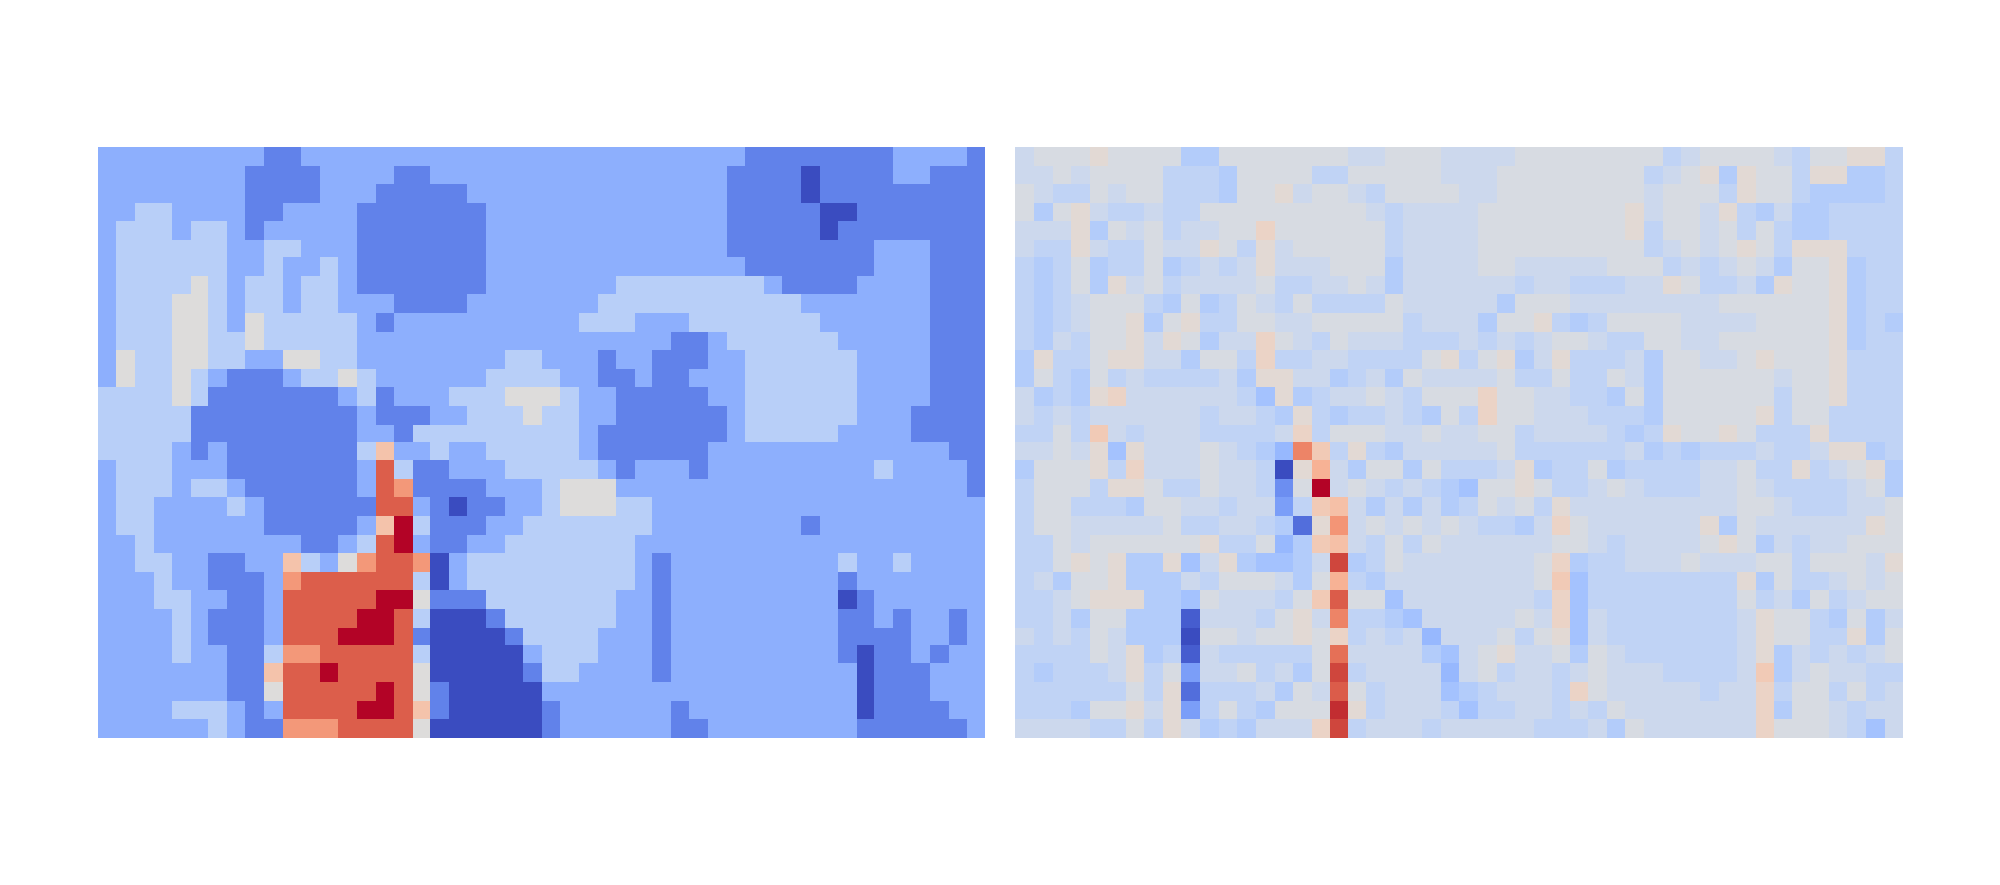
\includegraphics[width=.95\textwidth]{figures/kodim23_cb_components.pdf}
                \vspace{-12pt}
                \caption{$\bm{\mathcal{U}}_{C_B}$ channels}
            \end{subfigure}%
        \end{minipage}
        \begin{minipage}{\textwidth}
            \begin{subfigure}{\textwidth}
                \centering
                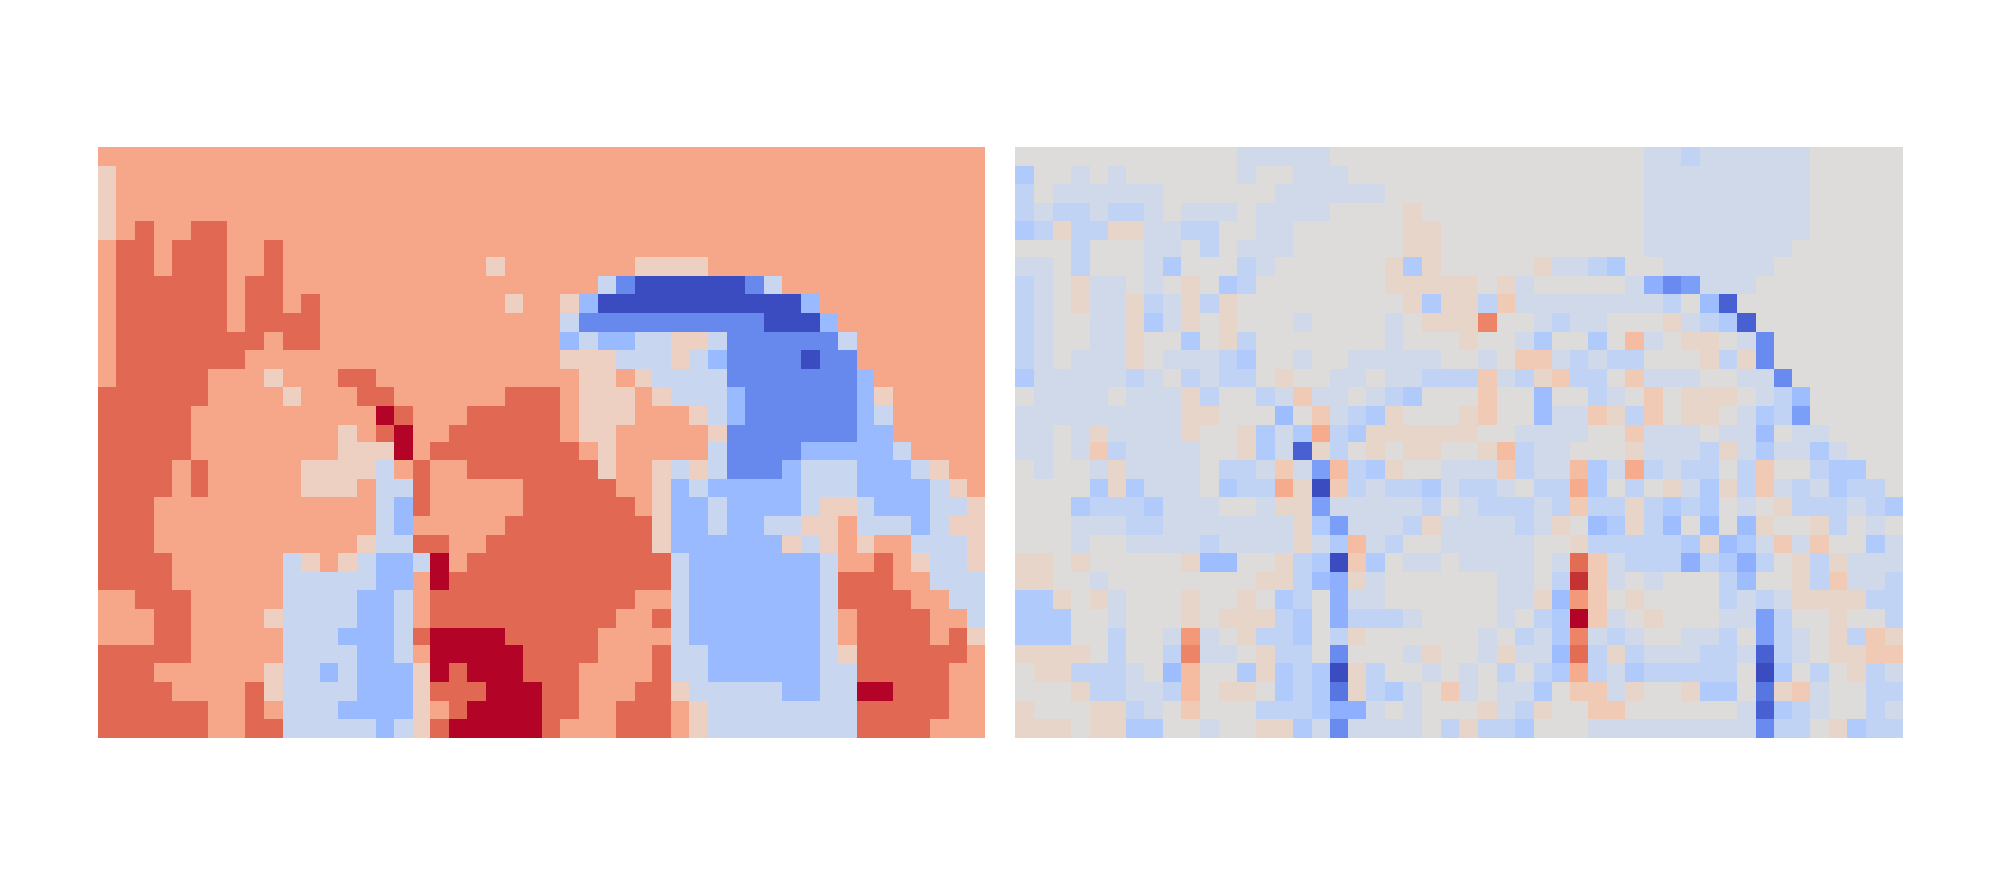
\includegraphics[width=.95\textwidth]{figures/kodim23_cr_components.pdf}
                \vspace{-12pt}
                \caption{$\bm{\mathcal{U}}_{C_R}$ channels}
            \end{subfigure}%
        \end{minipage}
    \end{minipage}
    \caption{The channels of IMF basis maps for the \texttt{kodim23} image from Kodak. corresponding to luma (a), blue-difference (b), and red-difference (c) chroma.}
	\label{fig: imf_components}
\end{figure}


\subsection{Decoding} \label{sec: decoding}

The decoder receives an encoded image and reconstructs the RGB image by applying the inverse of the operations used by the encoder, starting from the last layer and moving to the first. Initially, the factor maps defined in \eqref{eq: reshaped factors} are produced by losslessly decompressing the encoded image. These maps are then transformed into factor matrices by flattening their spatial dimensions. The matrices $\bm{X}_{Y}$, $\bm{X}_{C_B}$, and $\bm{X}_{C_R}$ are calculated through the product of the corresponding factor matrices due to \eqref{eq: lra}. The \emph{luma} and downsampled \emph{chroma} components are then obtained by reshaping $\bm{X}_{Y}$, $\bm{X}_{C_B}$, and $\bm{X}_{C_R}$ back into their spatial forms, following the inverse of the patchification step. Subsequently, the downsampled \emph{chroma} components are upsampled to their original size using bilinear interpolation. Finally, the YC\textsubscript{B}C\textsubscript{R} image is converted back into an RGB image. 

\subsection{Integer Matrix Factorization (IMF)} \label{sec: imf}

The main building block of our method is integer matrix factorization (IMF), which is responsible for the lossy compression of matrices obtained through patchification. IMF can be framed as an optimization problem, aiming to minimize the reconstruction error between the original matrix $\bm{X} \in \mathbb{R}^{M \times N}$ and the product $\bm{U} \bm{V}^\mathsf{T}$, while ensuring that the elements of the factor matrices $\bm{U}$ and $\bm{V}$ are integers within a specified interval $[\alpha,\beta]$ with integer values $\alpha$ and $\beta$, i.e., $\alpha,\beta\in\Z$. Formally, the IMF problem can be expressed as:
\begin{align} \label{eq: imf problem}
	\minimize_{\bm{U}, \bm{V}} & \ \  \| \bm{X} - \bm{U} \bm{V}^\mathsf{T} \|_\text{F}^2 \nonumber \\
	\text{s.t.}           & \ \ \bm{U} \in \mathbb{Z}_{[\alpha,\beta]}^{M \times R}, \bm{V} \in \mathbb{Z}_{[\alpha,\beta]}^{N \times R},
\end{align}
where $\|\cdot\|_\text{F}$ denotes the Frobenius norm; $R \leq \min(M,N)$ represents the \emph{rank}; and $\mathbb{Z}_{[\alpha,\beta]} \triangleq [\alpha,\beta] \cap \mathbb{Z}$ denotes the set of integers within $[\alpha,\beta]$. Without constraints on the factors, the problem would have an analytic solution through the singular value decomposition (SVD), as addressed by the Eckart–Young–Mirsky theorem \cite{eckart1936approximation}. If only a nonnegativity constraint were applied (without integrality), variations of nonnegative matrix factorization (NMF) would emerge \cite{lee2000algorithms, gillis2020nonnegative}. The IMF problem \eqref{eq: imf problem} poses a challenging integer program, with finding its global minima known to be NP-hard \cite{dong2018integer, van1981another}. Only a few iterative algorithms \cite{dong2018integer, lin2005integer} have been proposed to find a ``good solution'' for some IMF variants in contexts other than image compression. In Section \ref{sec: bcd}, we propose an efficient iterative algorithm for the IMF problem \eqref{eq: imf problem}.

The application of SVD and NMF in image compression is problematic mainly because the resulting factors contain continuous values that must be represented as arrays of floating-point numbers. This necessitates a quantization step that not only adds extra complications but also significantly degrades compression performance due to quantization errors (as demonstrated in Section \ref{sec: experiments}). Conversely, our IMF formulation produces integer factor matrices that can be directly stored and losslessly processed without incurring roundoff errors. The reason for limiting the feasible region to $[\alpha,\beta]$ in our IMF formulation is to enable more compact storage of the factors using standard integral data types, such as \texttt{int8} and \texttt{int16}, supported by programming languages. Given that the elements of the input matrix $\bm{X}$ are in $[0, 255]$, we found the signed \texttt{int8} type, which represents integers from -128 to 127, suitable for image compression applications. As a result, our IMF formulation is well-suited for image compression, effectively integrating the factorization and quantization steps into a single, efficient compression process.


\subsection{Block Coordinate Descent Scheme for IMF} \label{sec: bcd}

\begin{algorithm}[!t]
	\caption{The proposed block coordinate descent (BCD) algorithm for IMF. \label{alg: bcd for imf}}
	\DontPrintSemicolon
	\SetAlgoLined
	\KwIn{$\bm{X} \in \mathbb{R}^{M \times N}$, factorization rank $R$}
	\KwOut{Factor matrices $\bm{U} \in \mathbb{Z}_{[\alpha,\beta]}^{M \times R}$ and $\bm{V} \in \mathbb{Z}_{[\alpha,\beta]}^{N \times R}$}
	Initialize $\bm{U}^{\rm init}$, $\bm{V}^{\rm init}$ using the truncated SVD method, provided by \eqref{eq: initialization: u} and \eqref{eq: initialization: v}, and set $k=0$\;
	\While{stopping criterion not satisfied}{
        $k \gets k+1$\;
		$\bm{A} \gets \bm{X} \bm{V}^k$,\ $\bm{B} \gets \bm{V}^{k^{\mathsf{T}}} \bm{V}^k$\;
		\For{$r = 1, \ldots, R$}{
			$\displaystyle U_{:r}^{k+1} = \clamp_{[\alpha,\beta]}\Big(\round \Big(\frac{A_{:r} - \sum_{s = 1}^{r-1} B_{sr} U_{:s}^{k+1} - \sum_{s=r+1}^M B_{sr} U_{:s}^k}{\| V_{:r}^k \|^2}\Big)\Big)$\;
		}
		$\bm{A} \gets \bm{X}^\mathsf{T} \bm{U}^{k+1}$; $\bm{B} \gets \bm{U}^{{k+1}^\mathsf{T}} \bm{U}^{k+1}$\;
		\For{$r = 1, \ldots, R$}{
			$\displaystyle V_{:r}^{k+1} = \clamp_{[\alpha,\beta]}\Big(\round \Big(\frac{A_{:r} - \sum_{s = 1}^{r-1} B_{sr} V_{:s}^{k+1} - \sum_{s = r+1}^N B_{sr} V_{:s}^k}{\| U_{:r}^{k+1} \|^2}\Big)\Big)$\;
		}
	}
	\Return $(\bm{U}^k, \bm{V}^k)$
\end{algorithm}

We propose an efficient algorithm for IMF using the block coordinate descent (BCD) scheme (aka alternating optimization). 
The pseudocode is provided in Algorithm \ref{alg: bcd for imf}.
Starting with some initial parameter values, this approach involves sequentially minimizing the cost function with respect to a single column of a factor at a time, while keeping the other columns of that factor and the entire other factor fixed. This process is repeated until a stopping criterion is met, such as when the change in the cost function value falls below a predefined threshold or the maximum number of iterations is reached. Formally, this involves solving one of the following subproblems at a time:
\begin{align}  
	\bm{u}_r \gets \underset{\bm{u}_r \in \mathbb{Z}_{[\alpha,\beta]}^M}{\argmin} \ \lVert \bm{E}_r - \bm{u}_r \bm{v}_r^\mathsf{T} \rVert_\text{F}^2, \label{eq: bcd subproblem: u} \\
	\bm{v}_r \gets \underset{\bm{v}_r \in \mathbb{Z}_{[\alpha,\beta]}^N}{\argmin} \ \lVert \bm{E}_r - \bm{u}_r \bm{v}_r^\mathsf{T} \rVert_\text{F}^2, \label{eq: bcd subproblem: v}
\end{align}
where $\bm{u}_r \coloneqq U_{:r}$ and $\bm{v}_r \coloneqq V_{:r}$ represent the $r$-th columns of $\bm{U}$ and $\bm{V}$, respectively. $\bm{E}_r \coloneqq \bm{X} - \sum_{s \neq r}^{R} \bm{u}_s \bm{v}_s^\mathsf{T}$ is the residual matrix. We define one iteration of BCD as a complete cycle of updates across all the columns of both factors. In fact, the proposed algorithm is a $2R$-block coordinate descent procedure, where at each iteration, first the columns of $\bm{U}$ and then the columns of $\bm{V}$ are updated (see Algorithm \ref{alg: bcd for imf}). Note that subproblem \eqref{eq: bcd subproblem: v} can be transformed into the same form as \eqref{eq: bcd subproblem: u} by simply transposing its error term inside the Frobenius norm. Therefore, we only need to find the best rank-1 approximation with integer elements constrained within a specific interval. Fortunately, this problem has a closed-form solution, as addressed by Theorem \ref{the: bcd subproblem} below.

\begin{theorem}[Closed-form solutions] \label{the: bcd subproblem}
    The global optima of subproblems \eqref{eq: bcd subproblem: u} and \eqref{eq: bcd subproblem: v} can be represented by closed-form solutions. Specifically, these subproblems can be replaced by the following:
    \begin{align} 
            \textstyle \bm{u}_r \gets \clamp_{[\alpha,\beta]}\big(\round\big(\frac{\bm{E}_r \bm{v}_r}{\lVert \bm{v}_r \rVert^2}\big)\big), \label{eq: bcd_closed_form_subproblem_u}\\
            \textstyle \bm{v}_r \gets \clamp_{[\alpha,\beta]}\big(\round\big(\frac{\bm{E}_r^\mathsf{T} \bm{u}_r}{\lVert \bm{u}_r \rVert^2}\big)\big),             
        \label{eq: bcd_closed_form_subproblem_v}
    \end{align}
    where $\round(\bm{Z})$ denotes an element-wise operator that rounds each element of $\bm{Z}$ to the nearest integer, and $\clamp_{[\alpha,\beta]}(\bm{Z}) \triangleq \max(\alpha, \min(\bm{Z}, \beta))$ denotes an element-wise operator that clamps each element of $\bm{Z}$ to the interval $[\alpha,\beta]$.
\end{theorem}
\begin{proof}
	See Appendix \ref{app: monotonicity proof} for the proof.
\end{proof}

It is noteworthy that the combination of $\round(\cdot)$ and $\clamp_{[\alpha,\beta]}(\cdot)$ in \eqref{eq: bcd_closed_form_subproblem_u} and \eqref{eq: bcd_closed_form_subproblem_v} can be interpreted as the element-wise projector to $\mathbb{Z}_{[\alpha,\beta]}$. In Theorem \ref{thm:convergence}, the convergence of the proposed algorithm employing these closed-form solutions will be established.

\begin{theorem}[Global convergence]\label{thm:convergence}
    Let $\seq{\displaystyle U_{:r}^{k}}[k\in\N]$ and $\seq{\displaystyle V_{:r}^{k}}[k\in\N]$ for $r\in \{1,\dots,R\}$ be sequences generated by the proposed Algorithm \ref{alg: bcd for imf}. Then all sequences are bounded and convergent to a coordinatewise optimal point of optimization problem \eqref{eq: imf problem}.
\end{theorem}
\begin{proof}
    See Appendix \ref{app: convergence proof} for the proof.
\end{proof}




% \begin{theorem}[Integer rank-1 approximation] \label{the: bcd subproblem}
% 	Let $\bm{E} \in \mathbb{R}^{M \times N}$, $\bm{u} \in \mathbb{Z}_{[\alpha,\beta]}^{M \times 1}$, and $\bm{v} \in \mathbb{R}^{N \times 1}$. A global solution to the problem
% 	\begin{equation} \label{eq: bcd subproblem}
% 		\bm{u}^* \in \underset{\bm{u} \in \mathbb{Z}_{[\alpha,\beta]}^{M \times 1}}{\argmin} \ \lVert \bm{E} - \bm{u} \bm{v}^\mathsf{T} \rVert_\text{F}^2
% 	\end{equation}
% 	is given by
% 	\begin{equation} \label{eq: bcd subproblem solution}
% 		\bm{u}^* = \clamp_{[\alpha,\beta]}\Big(\round\Big(\frac{\bm{E} \bm{v}}{\lVert \bm{v} \rVert^2}\Big)\Big),
% 	\end{equation} 
% 	where $\round(\bm{Z})$ denotes the operator that rounds each element of $\bm{Z}$ to the nearest integer, and $\clamp_{[\alpha,\beta]}(\bm{Z}) \triangleq \max(\alpha, \min(\bm{Z}, \beta))$ denotes the operator that clamps each element of $\bm{Z}$ to the interval $[\alpha,\beta]$.
% \end{theorem}

% Using Theorem \ref{the: bcd subproblem}, we obtain the following update formulas for our BCD algorithm:
% Thanks to Theorem \ref{the: bcd subproblem}, the proposed algorithm offers an encouraging property that guarantees the cost function is monotonically non-increasing with each update. 


\paragraph{Initialization.}
The initial values of factors can significantly impact the convergence performance of the BCD algorithm. We found that the convergence with naive random initialization can be too slow. To address this issue, we propose an initialization method using SVD. The procedure is straightforward. First, the truncated SVD of the input matrix $\bm{X} \in \mathbb{R}^{M \times N}$ is computed as $\tilde{\bm{U}} \bm{\Sigma} \tilde{\bm{V}}^\mathsf{T}$, where $\bm{\Sigma} \in \mathbb{R}^{R \times R}$ is a diagonal matrix corresponding to the $R$ largest singular values. $\tilde{\bm{U}} \in \mathbb{R}^{M \times R}$ contains the corresponding left-singular vectors in its columns, and $\tilde{\bm{V}} \in \mathbb{R}^{N \times R}$ contains the corresponding right-singular vectors in its columns. The initial factors are then calculated as follows:
\begin{align} 
	\bm{U}^{\rm init} = \clamp_{[\alpha,\beta]}(\round(\tilde{\bm{U}} \bm{\Sigma}^\frac{1}{2})), \label{eq: initialization: u} \\
	\bm{V}^{\rm init} = \clamp_{[\alpha,\beta]}(\round(\bm{\Sigma}^\frac{1}{2} \tilde{\bm{V}})). \label{eq: initialization: v}
\end{align}
Essentially, this means we first low-rank approximate $\bm{X}$ and then project the elements of the resulting factor matrices into $\mathbb{Z}_{[\alpha,\beta]}$. 



\section{Experiments} \label{sec: experiments}

In this section, the proposed IMF compression algorithm is assessed against baseline codecs following the implementation details.
Moreover, ablation studies are presented to investigate the effect of different parameters in IMF.

\subsection{Qualitative Performance}
% The first channels of factor maps $\bm{\mathcal{U}}_{Y}, \bm{\mathcal{U}}_{C_B}$ and $\bm{\mathcal{V}}_{Y}$ defined in \eqref{eq: reshaped factors} are depicted in Figure \ref{fig:imf_components} for an image selected from the Kodak dataset. 
% It is evident that each channel of factor maps can be treated as an 8-bit grayscale image in the lossless compression stage of the encoder. The channels with higher energy maintain the overall texture of the original image, while channels with lower energy focus more on subtle changes. 

The qualitative comparison is made in Figure \ref{fig:qualitative_comparison} where the compressed images by different algorithms are shown in different bpp values.
As can be seen, the proposed IMF compression algorithm is capable of maintaining quality compressed images in bpp values as low as $0.15$, outperforming JPEG and SVD-based methods which suffer from maintaining balanced colors in low bpp values. 
The artifacts in color produced by JPEG are visible in both example images.
\begin{figure}[t]
	\centering
	\begin{subfigure}{.23\textwidth}
		\centering
        \text{\small Original image}
		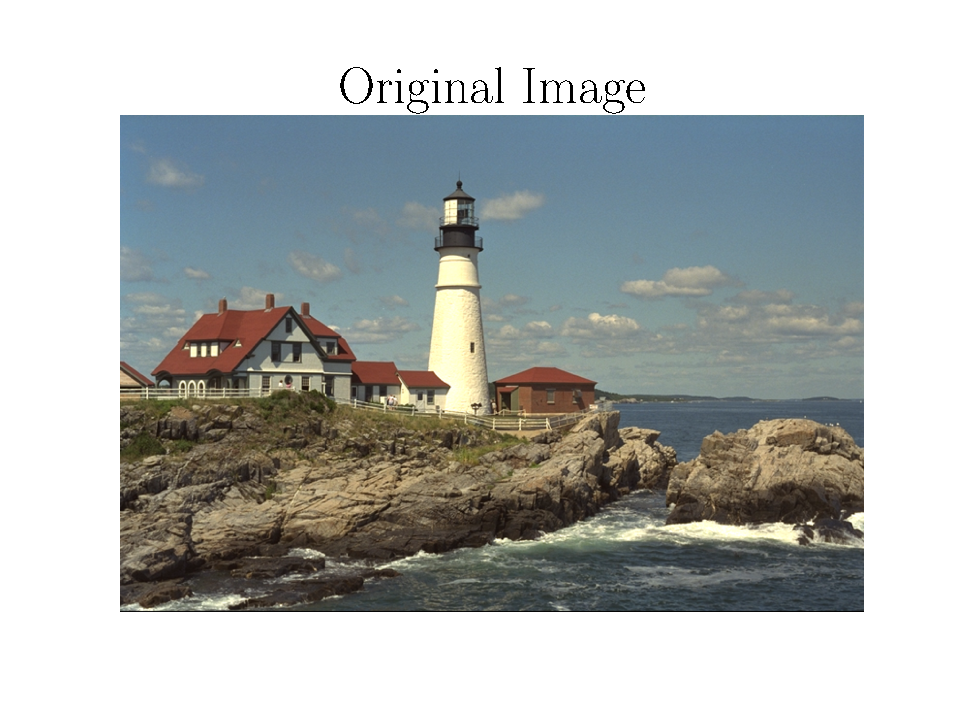
\includegraphics[trim=1.7cm 1.5cm 1.7cm 1.7cm, clip, width=1\textwidth]{figures/kodim21_original.pdf}
        \vspace{-20pt}
        \caption*{}
	\end{subfigure}%
	\begin{subfigure}{.23\textwidth}
		\centering
        \text{\small JPEG}
		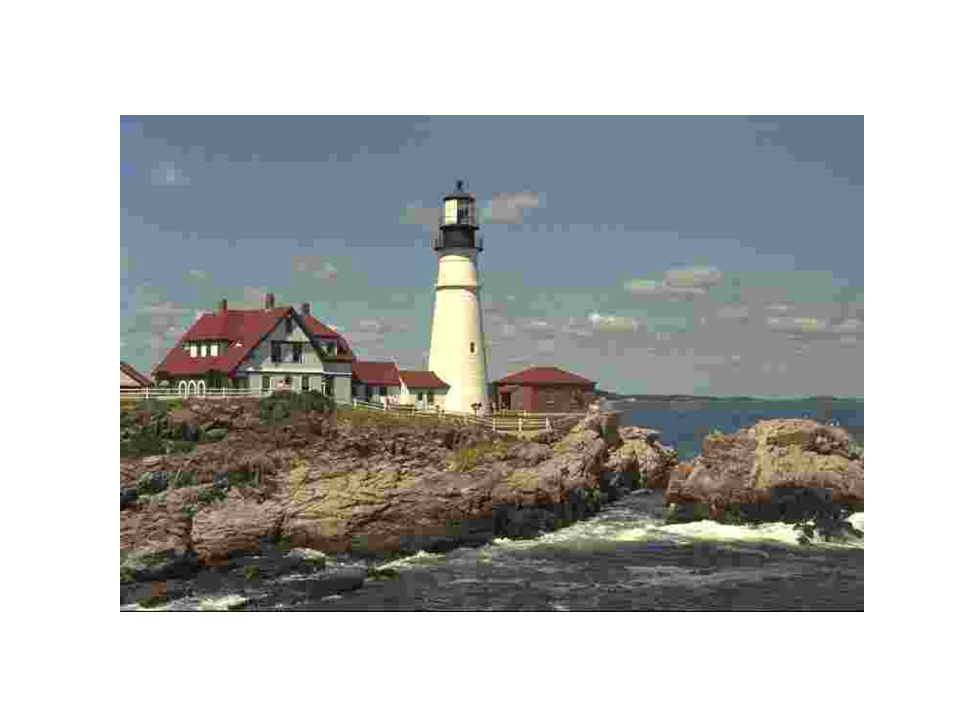
\includegraphics[trim=1.7cm 1.5cm 1.7cm 1.7cm, clip, width=1\textwidth]{figures/kodim21_JPEG_bpp_0.293.pdf}
        \vspace{-20pt}
        \caption*{\tiny \textbf{PSNR: 25.40 ~ bpp: 0.29}}
	\end{subfigure}
    \begin{subfigure}{.23\textwidth}
		\centering
        \text{\small SVD}
		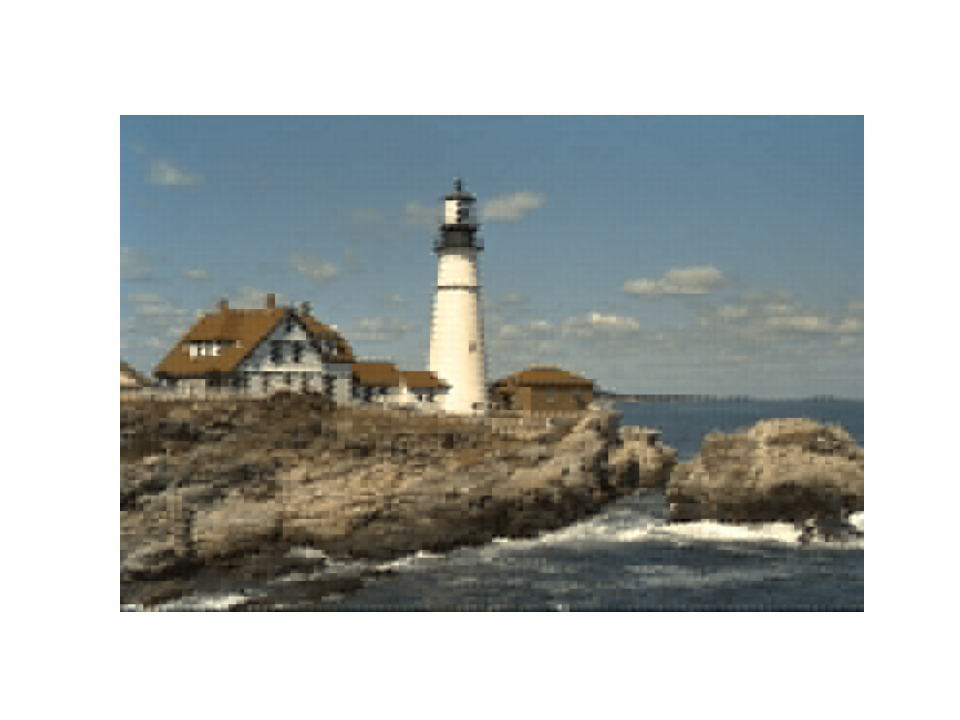
\includegraphics[trim=1.7cm 1.5cm 1.7cm 1.7cm, clip, width=1\textwidth]{figures/kodim21_SVD_bpp_0.315.pdf}
        \vspace{-20pt}
        \caption*{\tiny \textbf{PSNR: 23.62 ~ bpp: 0.31}}
	\end{subfigure}
    \begin{subfigure}{.23\textwidth}
		\centering
        \text{\small IMF}
		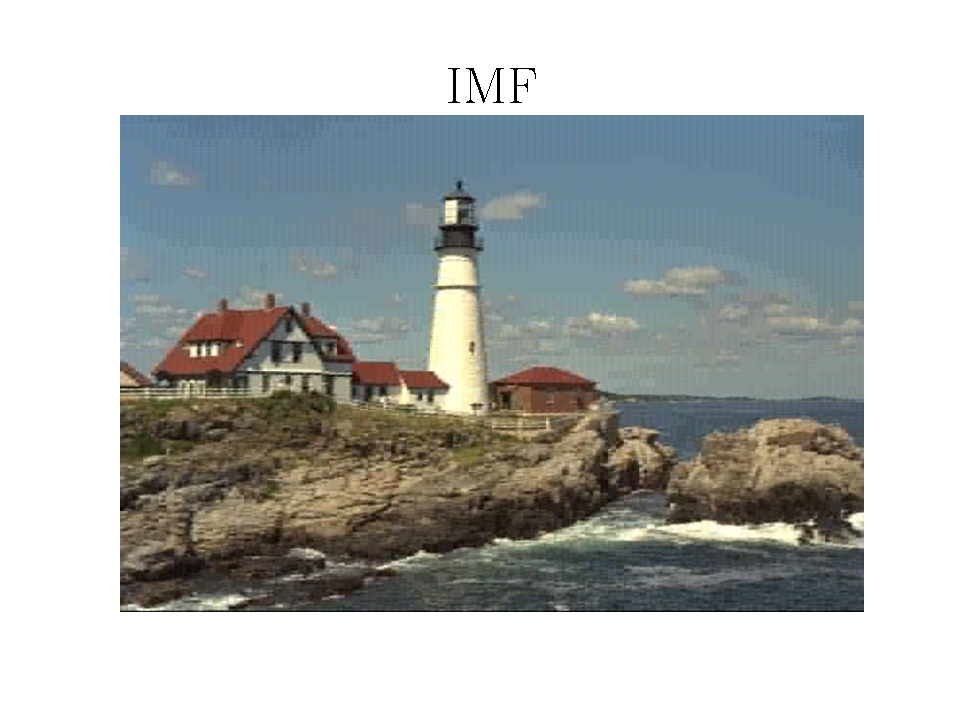
\includegraphics[trim=1.7cm 1.5cm 1.7cm 1.7cm, clip, width=1\textwidth]{figures/kodim21_IMF_bpp_0.305.pdf}
        \vspace{-20pt}
        \caption*{\tiny \textbf{PSNR: 25.71 ~ bpp: 0.30}}
	\end{subfigure}


	\begin{subfigure}{.23\textwidth}
		\centering
		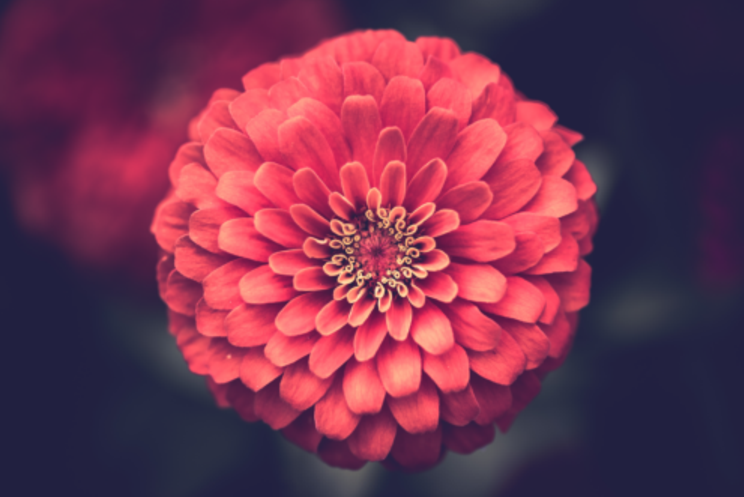
\includegraphics[trim=1.7cm 1.5cm 1.7cm 1.7cm, clip, width=1\textwidth]{figures/clic_flower_original.pdf}
        \vspace{-20pt}
        \caption*{}
	\end{subfigure}%
	\begin{subfigure}{.23\textwidth}
		\centering
		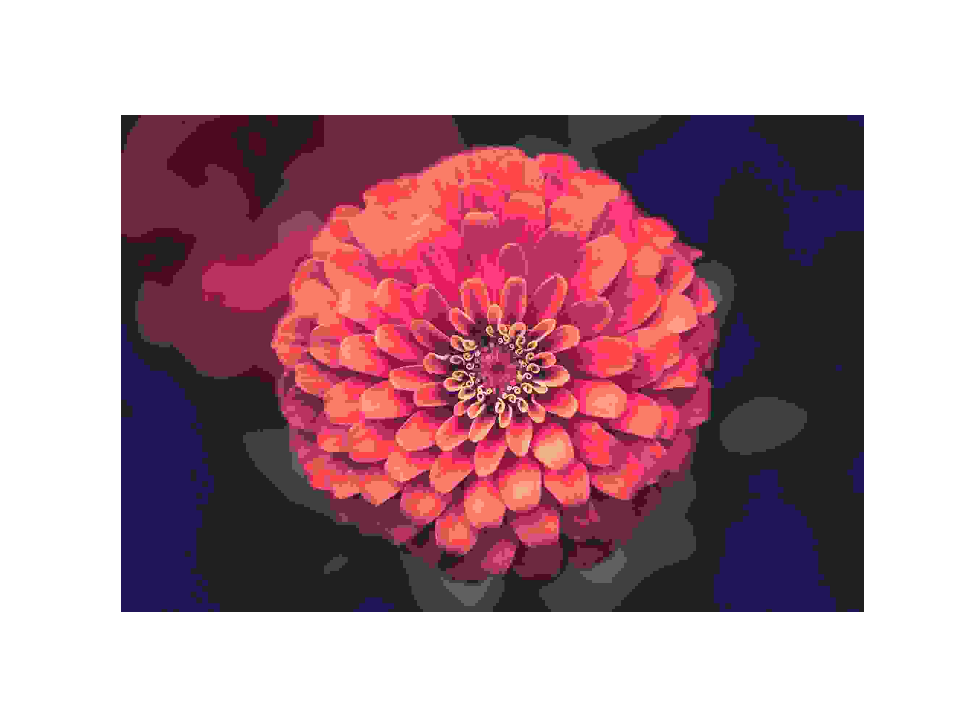
\includegraphics[trim=1.7cm 1.5cm 1.7cm 1.7cm, clip, width=1\textwidth]{figures/clic_flower_JPEG_bpp_0.137.pdf}
        \vspace{-20pt}
        \caption*{\tiny \textbf{PSNR: 22.65 ~ bpp: 0.13}}
	\end{subfigure}
    \begin{subfigure}{.23\textwidth}
		\centering
		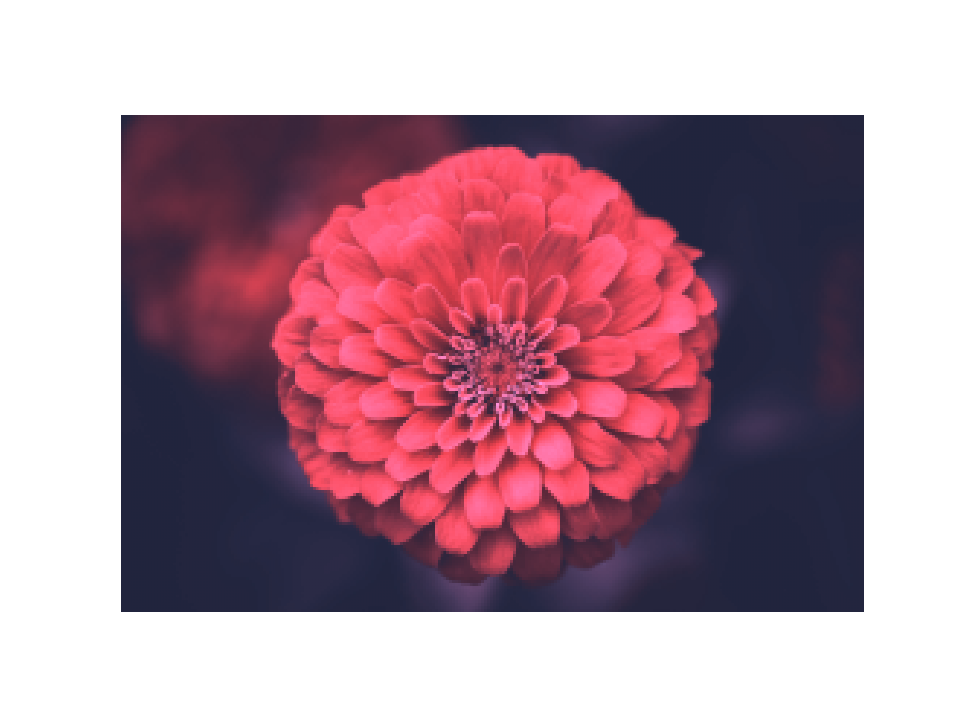
\includegraphics[trim=1.7cm 1.5cm 1.7cm 1.7cm, clip, width=1\textwidth]{figures/clic_flower_SVD_bpp_0.123.pdf}
        \vspace{-20pt}
        \caption*{\tiny \textbf{PSNR: 26.85 ~ bpp: 0.12}}
	\end{subfigure}
    \begin{subfigure}{.23\textwidth}
		\centering
		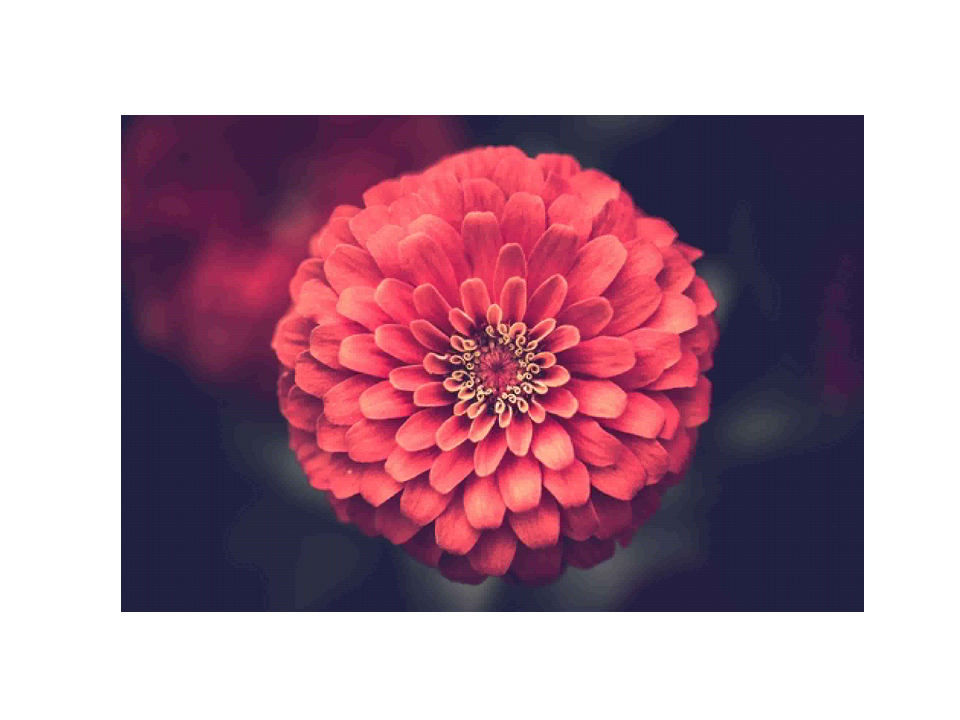
\includegraphics[trim=1.7cm 1.5cm 1.7cm 1.7cm, clip, width=1\textwidth]{figures/clic_flower_IMF - YCbCr_bpp_0.108.pdf}
        \vspace{-20pt}
        \caption*{\tiny \textbf{PSNR: 31.73 ~ bpp: 0.10}}
	\end{subfigure}

    \caption{Qualitative performance comparison on an image from Kodak (top row) and CLIC (bottom row).}
	\label{fig:qualitative_comparison}
\end{figure}



\subsection{Rate-Distortion Performance} \label{sec:rate_distortion_performance}
In this section, we plot the PSNR-bpp curves for each algorithm to compare their compression performance. The corresponding SSIM-bpp curves are postponed to the appendix.
In the figures, for each compressed image, bpp and PSNR values are calculated. Then, for each compression method, PSNR values are interpolated linearly in some fixed bpp values in the range $(0.05, 0.5)$. 
In the following plots, the average performance over all images is reported, along with the standard deviation which is presented as shadows.
For the missing bpp values, the average is extrapolated quadratically and is shown by dashed lines.

In Figure \ref{fig:compression_performance_kodak_clic}, the compression performance on the Kodak and CLIC datasets is reported. 
In this figure, the proposed IMF compression algorithm outperforms the SVD-based compression, which can be attributed to the quantization errors that SVD is prone to during encoding and decoding, deteriorating its performance. In this view, the quantization-free property of IMF effectively guarantees higher performance in different bpp values.
It is also evident that the IMF compression algorithm outperforms JPEG in low bpp values.
\begin{figure}[t]
	\centering
	\begin{subfigure}{.45\textwidth}
		\centering
		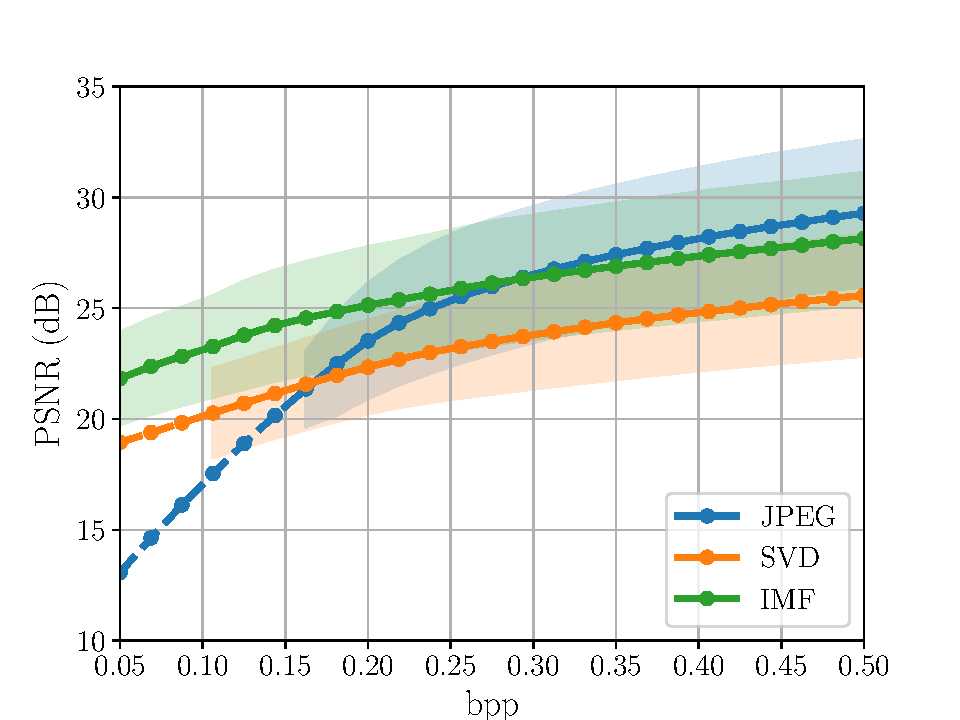
\includegraphics[width=.95\textwidth]{figures/comparison_kodak_psnr.pdf}
		\caption{performance on Kodak}
		\label{fig: psnr-vs-bpp kodak}
	\end{subfigure}%
	\begin{subfigure}{.45\textwidth}
		\centering
		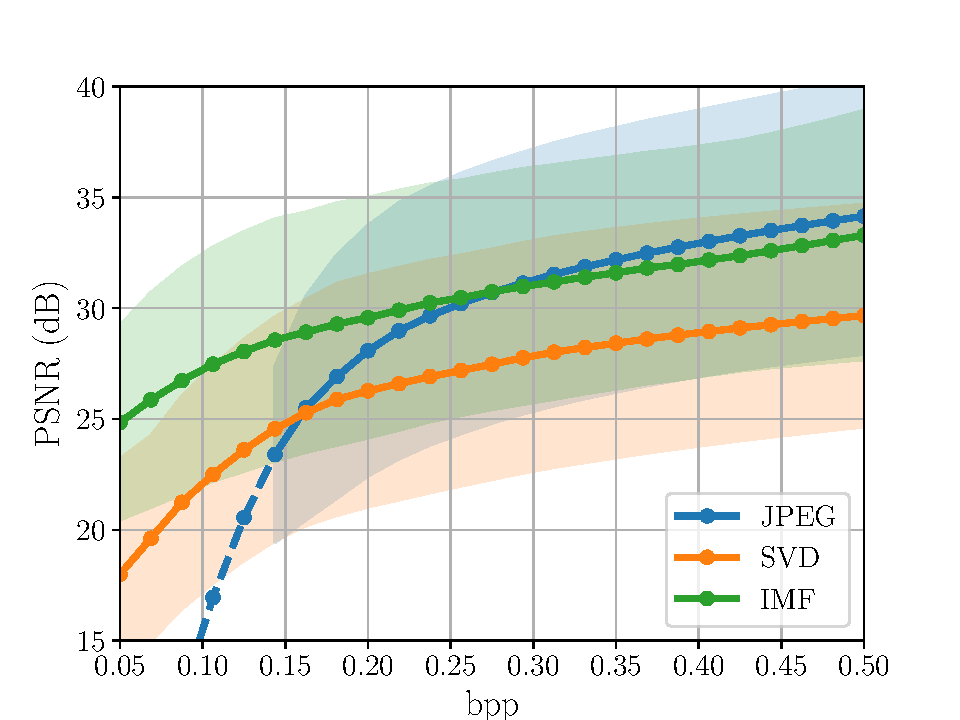
\includegraphics[width=.95\textwidth]{figures/comparison_clic_psnr.pdf}
		\caption{performance on CLIC}
		\label{fig: psnr-vs-bpp clic}
	\end{subfigure}
	\caption{Performance comparison of JPEG, SVD, and IMF compression algorithms on Kodak and CLIC. 
    % The average PSNR of compressed images is reported in different bpps values in the range $[0.05,0.5]$.
    }
	\label{fig:compression_performance_kodak_clic}
\end{figure}

\subsection{ImageNet Classification Performance} \label{sec: imagenet Classification Performance}
As another criterion, we investigate the performance of an image classifier on the images compressed by different compression algorithms. 
This criterion focuses on the capability of different compression methods to preserve the visual semantic information in each image.
Furthermore, it highlights the importance of image compression where various vision tasks such as classification---rather than maintaining the perceived image quality---are the main objective, while keeping the requirement of resources such as memory, communication bandwidth, computation power, latency budget, etc. as limited as possible.
ImageNet \cite{deng2009imagenet} validation set, consisting of 50000 $224 \times 224$ RGB images in 1000 classes, is considered in this classification task done by a ResNet-50 classifier \cite{he2016deep}, pre-trained on the original ImageNet dataset.
The classification performance comparison is made in Figure \ref{fig:imagenet_classification}. 
The results suggest that IMF leads to more than a $25\%$ relative improvement in top-1 accuracy over JPEG at the low bitrate of 0.23 bpp and reaches top-5 accuracy of more than $70\%$ at the bpp value of 0.2. 


\begin{figure}[t]
	\centering
	\begin{subfigure}{.45\textwidth}
		\centering
				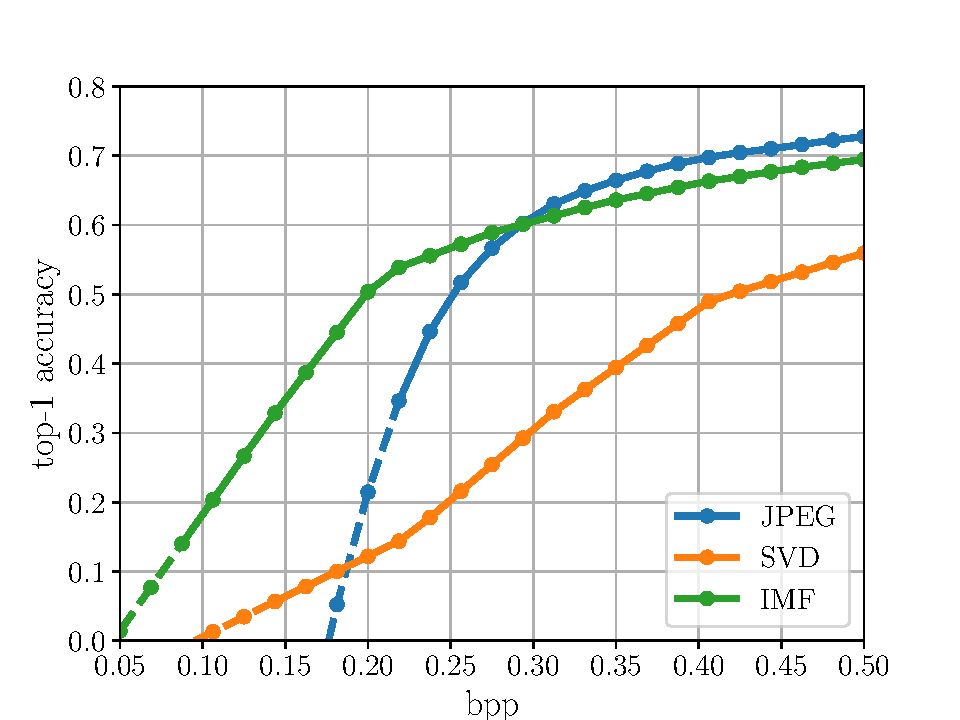
\includegraphics[width=.95\textwidth]{figures/classification_performance_top1.pdf}
		\caption{top-1 accuracy}
		\label{fig: top1-vs-bpp imagenet}
	\end{subfigure}%
	\begin{subfigure}{.45\textwidth}
		\centering
				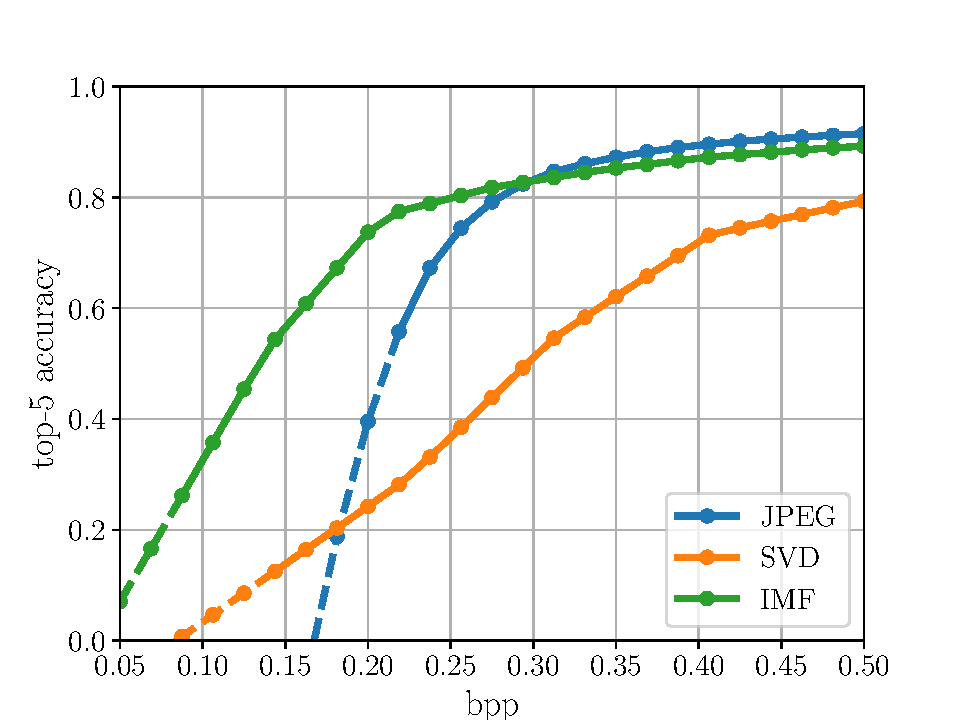
\includegraphics[width=.95\textwidth]{figures/classification_performance_top5.pdf}
		\caption{top-5 accuracy}
		\label{fig: top5-vs-bpp imagenet}
	\end{subfigure}
	\caption{Impact of different compression methods on ImageNet classification accuracy. 
    % Panels (a) and (b) show the validation top-1 and top-5 accuracy plotted against bpp, respectively. 
    A ResNet-50 classifier, pre-trained on the original ImageNet images, is evaluated using validation images compressed by different methods.}
	\label{fig:imagenet_classification}
\end{figure}


\subsection{Ablation Studies} \label{sec: ablation studies}
In this section, ablation studies are performed, focusing on factor bounds and BCD iteration numbers in the proposed IMF compression algorithm and their effect on its performance. The other ablation studies are postponed to the appendix.

\paragraph{Factor bounds.} 
Figure \ref{fig: bounds ablation psnr-vs-bpp} studies the compression performance of IMF with different factor bounds $\alpha$ and $\beta$ in Algorithm \ref{alg: bcd for imf}. According to the results, the bounds $\alpha=-16$ and $\beta=15$ lead to the best performance. Limiting factor elements within these bounds leads to dedicating fewer bits to represent the resulting narrower range, compared to the other bounds, and consequently higher compression rates without sacrificing performance. 

\paragraph{BCD iteration.}
The next parameter to study is the maximum iteration number specified for the BCD updates of IMF in Algorithm \eqref{alg: bcd for imf}. 
According to the numerical results on various datasets, the IMF performance jumps significantly after 2 iterations, while more iteration numbers lead to marginal improvement. 
This observation is shown for Kodak in Figure \ref{fig: iteration ablation psnr-vs-bpp}.
This feature makes IMF computationally efficient since with a limited number of BCD iterations a high compression performance can be achieved.


\begin{figure}[t]
	\centering
	% \begin{subfigure}{.5\textwidth}
	% 	\centering
	% 	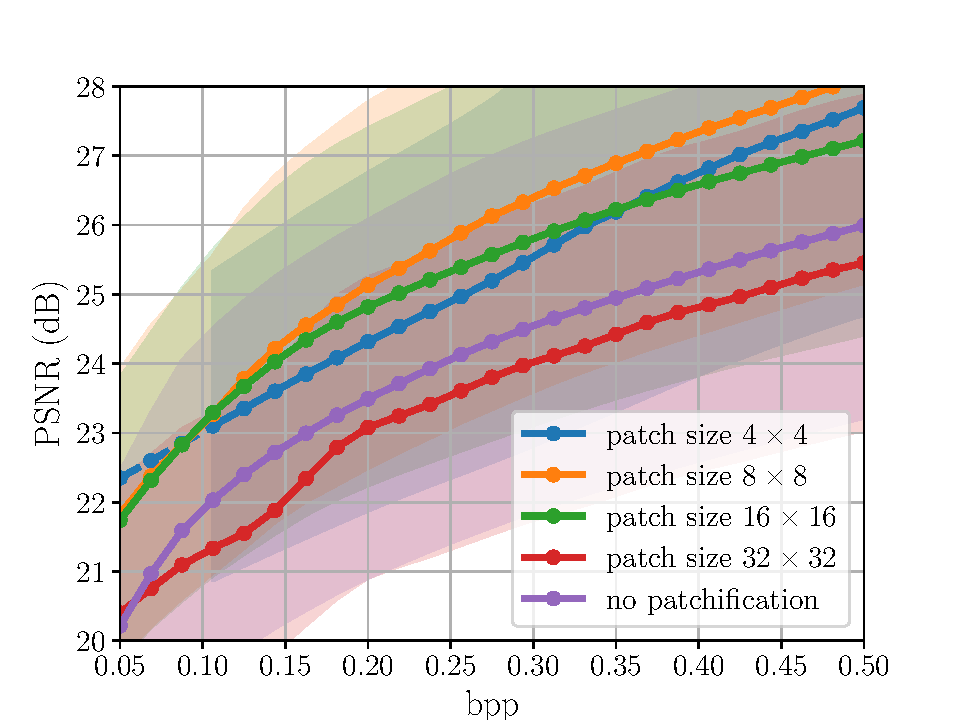
\includegraphics[width=.95\textwidth]{figures/ablation_patchsize_psnr.pdf}
	% 	\caption{}
	% 	\label{fig: patch ablation psnr-vs-bpp}
	% \end{subfigure}%
	\begin{subfigure}{.45\textwidth}
		\centering
		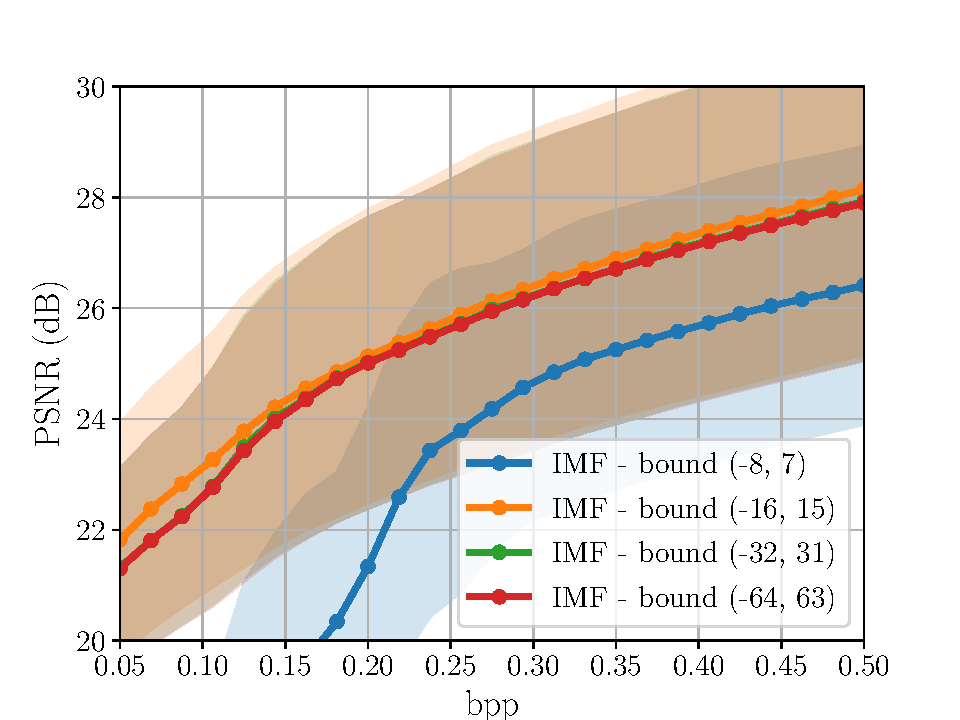
\includegraphics[width=.95\textwidth]{figures/ablation_bounds_psnr.pdf}
		\caption{ablation on factor bounds}
		\label{fig: bounds ablation psnr-vs-bpp}
	\end{subfigure}
    \begin{subfigure}{.45\textwidth}
		\centering
		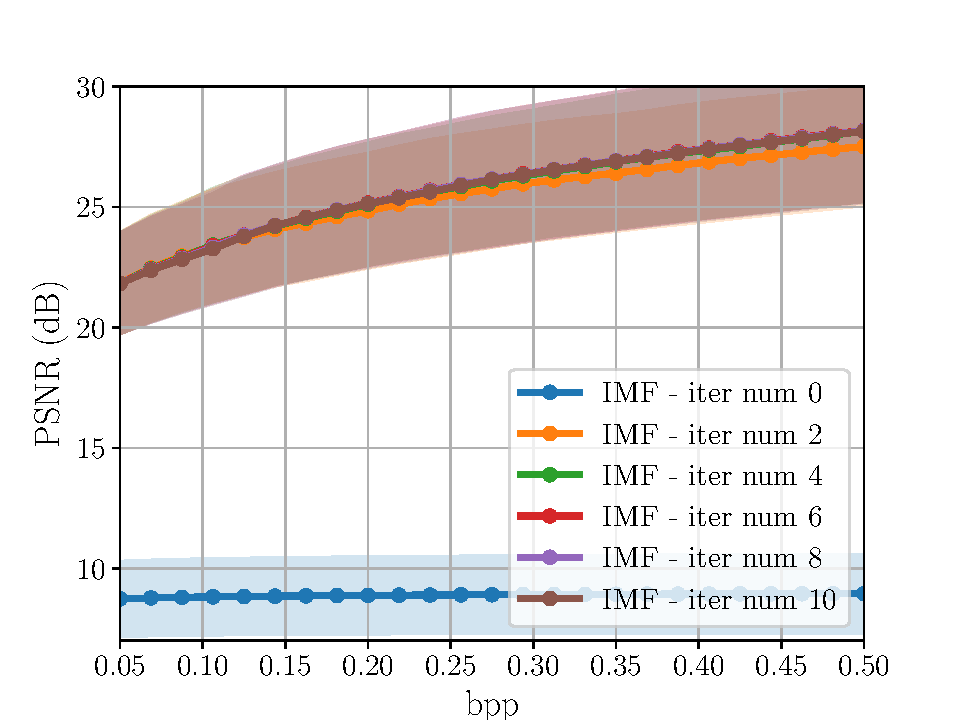
\includegraphics[width=.95\textwidth]{figures/ablation_iternum_psnr.pdf}
		\caption{ablation on BCD iteration number}
		\label{fig: iteration ablation psnr-vs-bpp}
	\end{subfigure}%
	% \begin{subfigure}{.5\textwidth}
	% 	\centering
	% 	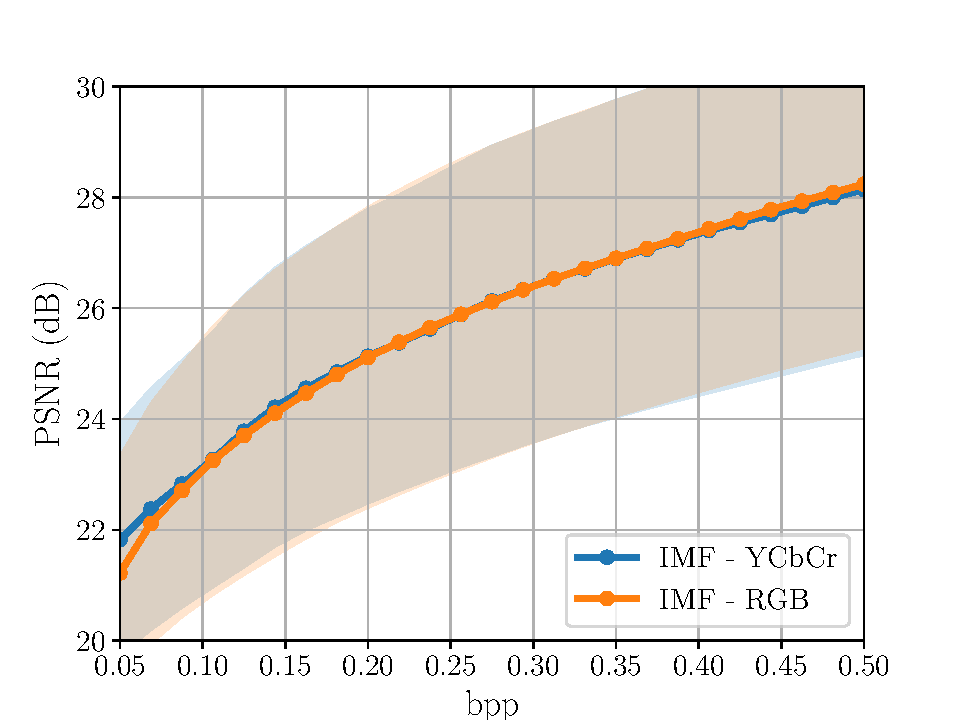
\includegraphics[width=.95\textwidth]{figures/ablation_colorspace_psnr.pdf}
	% 	\caption{}
	% 	\label{fig: colorspace ablation psnr-vs-bpp}
	% \end{subfigure}
	\caption{Ablation studies for IMF. Average PSNR on the Kodak dataset is reported versus bpp. 
    % In all cases, we plot PSNR as a function of bits per pixel (bpp) on the Kodak dataset. 
    % (a) Compares IMF compression performance without patchification and different patch sizes. 
    % (b) Compares IMF compression performance for different bound values of factor matrices. 
    % (c) Compares IMF compression performance for different numbers of BCD iterations. 
    % (d) Compares IMF compression performance between RGB and YCbCr color space transform.
    }
	\label{fig: ablation studies}
\end{figure}




\section{Conclusion} \label{sec:conclusion}

This work presents a novel quantization-free lossy image compression method based on integer matrix factorization (IMF). By representing image data as a product of two smaller matrices with bounded integer elements, the proposed IMF approach effectively eliminates the need for quantization, a significant source of error in traditional compression methods like JPEG and SVD. The reshaped factor matrices are compatible with existing lossless compression standards, enhancing the overall efficiency and flexibility of the \remove{system}\revise{method}. Our proposed iterative algorithm, utilizing a block coordinate descent scheme, has proven to be both efficient and convergent. Experimental results demonstrate that the IMF method significantly outperforms JPEG in terms of PSNR and SIMM at low bit rates and maintains better visual semantic information. This advantage underscores the potential of IMF to set a new standard in lossy image compression, bridging the gap between factorization and quantization.

\remove{A limitation of IMF lies in its inability to control the entropy of the elements in the factor matrices, which could enhance the performance of the subsequent entropy-based lossless coder. We plan to address this in the future by incorporating entropy-aware regularization into the current IMF objective function.}

\section*{Acknowledgments}

This research received funding from the Flemish Government (AI Research Program). Sabine Van Huffel and Pooya Ashtari are affiliated to Leuven.AI - KU Leuven institute for AI, B-3000, Leuven, Belgium.


\medskip

{
\small
\bibliographystyle{plainnat}
\bibliography{ref}
}


%%%%%%%%%%%%%%%%%%%%%%%%%%%%%%%%%%%%%%%%%%%%%%%%%%%%%%%%%%%%

\appendix

\section{Proof of Theorem \ref{the: bcd monotonicity}} \label{app: proof}

\begin{theorem}[Global convergence]
    Let $\seq{\bm U^k}[k\in\N]$ and $\seq{\bm V^k}[k\in\N]$ be sequences generated by the proposed Algorithm \ref{alg:lrf:hals for nmf}. Then both sequences are convergent to a locally optimal point of the optimization problem \eqref{eq: imf problem}.
\end{theorem}

\begin{proof}
    To study the convergence of the proposed Algorithm \ref{alg:lrf:hals for nmf}, we recast the optimization problem \eqref{eq: imf problem} to the following equivalent problem:
    \begin{align}
        \begin{split}
            \minimize_{\bm U \in \R^{M\times R}, \bm V \in \R^{N\times R}} \Psi(\bm U, \bm V) &\coloneqq H(\bm U, \bm V) + f(\bm U) + g(\bm V),\\
            \text{where} \quad~~~ H(\bm U, \bm V) &\coloneqq \|\bm X - \bm U \bm V^{\rm T} \|_{\rm F}^2,\\
            f(\bm U) &\coloneqq \delta_{[a,b]}(\bm U) + \delta_\Z(\bm U),\\
            g(\bm V) &\coloneqq \delta_{[a,b]}(\bm V) + \delta_\Z(\bm V),
        \end{split}
        \label{eq:IMF_surrogate}
    \end{align}
    with $\delta_\mathcal{B}(\cdot)$ as the indicator function of the nonempty set $\mathcal{B}$ where $\delta_\mathcal{B}(\bm x) = 0$ if $\bm x \in \mathcal{B}$ and $\delta_\mathcal{B}(\bm x) = +\infty$, otherwise. By the definition of functions above, it is easy to confirm that the problems \eqref{eq: imf problem} and \eqref{eq:IMF_surrogate} are equivalent.
    
    The unconstrained optimization problem \eqref{eq:IMF_surrogate} consists of the sum of a differentiable (smooth) convex function $H$ with nonsmooth nonconvex functions $f$ and $g$. This problem has been extensively studied in the literature under the class of unconstrained nonconvex nonsmooth minimization problems. 
    One of the common algorithms applied to such a problem class is the well-known forward-backward-splitting (FBS) []. 
    In Algorithm \ref{alg:lrf:hals for nmf}, the variables $\bm U$ and $\bm V$ are updated sequentially following block coordinate (BC) descent minimization algorithms, also often called Gauss-Seidel updates or alternating minimization.
    Hence, in this convergence study we are interested in the algorithms that allow BC-type updates for the nonconvex nonsmooth problem of \eqref{eq:IMF_surrogate} []. Specifically, we focus on the proximal alternating linearized minimization (PALM) algorithm, relating its convergence behavior to that of Algorithm \ref{alg:lrf:hals for nmf}. 
    To that end, we show that the updates of Algorithm \ref{alg:lrf:hals for nmf} are equivalent to the updates of PALM on the recast problem of \eqref{eq:IMF_surrogate}, and all the assumptions necessary for the convergence of PALM is satisfied by our problem setting. 

    The PALM algorithm [] can be summarized as follows:
    \begin{enumerate}
        \item Initialize $\bm U^0 \in \R^{M\times R}$, $\bm V^0 \in \R^{N\times R}$ 
        \item For each iteration $k=0,1,...$ 
        \begin{align}
            \begin{split}
                \mysubnumber\quad \bm U^{k+1} &\in \prox^f_{c_k} \left(\bm U^k - \frac{1}{c_k} \nabla_{\bm U} H(\bm U^k, \bm V^k)\right), ~\text{with}~ c_k > L_1(\bm V^k)\\
                \mysubnumber\quad \bm V^{k+1} &\in \prox^g_{d_k} \left(\bm V^k - \frac{1}{d_k} \nabla_{\bm V} H(\bm U^{k+1}, \bm V^k)\right), ~\text{with}~ d_k > L_2(\bm U^{k+1})
            \end{split}
            \label{eq:palm_updates}
        \end{align}
    \end{enumerate}
    where the proximal map for an extended proper lower semicontinuous (nonsmooth) function $\func{\varphi}{\R^n}{(-\infty,+\infty]}$ and $\gamma > 0$ is defined as $\prox^\varphi_\gamma(\bm x) \coloneqq \argmin_{\bm w\in\R^n}\left\{\varphi(\bm w) + \frac{\gamma}{2} \|\bm w - \bm x\|^2_2\right\}$, $\nabla_x$ is the partial derivative with respect to $x$, and $L_1 > 0$, $L_2 > 0$ are local Lipschitz moduli, defined in the following assumption II.

    The following proposition investigates the necessary assumptions for convergence of PALM and Algorithm \ref{alg:lrf:hals for nmf}.
    \begin{prop}[Meeting required assumptions]\label{prop:assumptions}
        The assumptions necessary for the convergence of iterations in \eqref{eq:palm_updates} are satisfied by the functions involved in the problem \eqref{eq:IMF_surrogate}, specifically:
        \begin{enumerate}
            \item The indicator functions $\delta_{[a,b]}$ and $\delta_\Z$ are proper and lower semicontinuous functions, so do the functions $f$ and $g$;
            \item For any fixed $\bm V$, the partial gradient $\nabla_{\bm U} H(\bm U, \bm V)$ is globally Lipschitz continuous with modulus $L_1(\bm V) = \|\bm V^T \bm V\|_F$ defined by
            \begin{equation*}
                \|\nabla_{\bm U} H(\bm U_1, \bm V) - \nabla_{\bm U} H(\bm U_2, \bm V)\| \leq L_1(\bm V) \|\bm U_1 - \bm U_2\|, \quad \forall \bm U_1,\bm U_2 \in \R^{M\times R},
            \end{equation*}
            where $\|\cdot\|$ in this section denotes the $\ell_2$-norm of the vectorized input with the proper dimension (here, with the input in $\R^{MR\times 1}$).
            The similar Lipschitz continuity is evident for $\nabla_{\bm V} H(\bm U, \bm V)$ as well with modulus $L_2(\bm U) = \|\bm U \bm U^T\|_F$.
            \item The sequences $\bm U^k$ and $\bm V^k$ are bounded due to the indicator functions $\delta_{[a,b]}$ with bounded $a$ and $b$. Hence the moduli $L_1(\bm V^k)$ and $L_2(\bm U^k)$ are bounded from below and from above for all $k\in\N$.
            \item The function $H$ is twice differentiable, hence, its full gradient $\nabla H(\bm U,\bm V)$ is Lipschitz continuous on the bounded set $\bm U \in [a,b]^{M\times R}$, $\bm V \in [a,b]^{N\times R}$. Namely, with $M > 0$:
            \begin{align}
                \begin{split}
                    \|(\nabla_{\bm U} H(\bm U_1, \bm V_1) - \nabla_{\bm U} H(\bm U_2, \bm V_2), \nabla_{\bm V} H(\bm U_1, \bm V_1) - &\nabla_{\bm V} H(\bm U_2, \bm V_2))\| \\
                    &\leq M \|(\bm U_1 - \bm U_2, \bm V_1 - \bm V_2)\|,
                \end{split}
            \end{align}
            where $(\cdot,\cdot)$ denotes the concatination of the two arguments.
            \item The sets $[a,b]$ and integer numbers are semi-algebraic; so are their indicator functions. The function $H$ is also polynomial, hence it is semi-algebraic. The sum of these functions results in a semi-algebraic function $\Psi$ in \eqref{eq:IMF_surrogate}, hence $\Psi$ is a KL function.
        \end{enumerate}
    \end{prop}
    By Proposition \ref{prop:assumptions}, the optimization problem \eqref{eq:IMF_surrogate}---and equivalently the original problem \eqref{eq: imf problem}---can be solved by PALM, which is convergence to a locally optimal point, specifically a critical point $(\bm U^\star, \bm V^\star)$ where $0 \in \partial \Psi(\bm U^\star, \bm V^\star)$, with $\partial$ as the subdifferential of $\Psi$.

    In the following, we highlight that the updates in () can be implemented more simply and more efficiently by Algorithm \ref{alg:lrf:hals for nmf} for the problem of image compression. It is noted that the so-called \emph{forward} steps $\bm U^k - \frac{1}{c_k} \nabla_{\bm U} H(\bm U^k, \bm V^k)$ and $\bm V^k - \frac{1}{d_k} \nabla_{\bm V} H(\bm U^{k+1}, \bm V^k)$ in the $\prox$ operators can be replaced by the simple closed-form updates of Algorithm \ref{alg:lrf:hals for nmf} in steps () and (), respectively. This is thanks to the special form of the functions $H(\cdot, \bm V^k)$ and $H(\bm U^{k+1}, \cdot)$ being quadratic functions, each having a global optimal point which ensures a descent in each forward step. 
    Furthermore, the proximal operators $\prox^f_{c_k}$ and $\prox^g_{d_k}$ can efficiently be implemented by the steps () and () in Algorithm \ref{alg:lrf:hals for nmf}. The equivalence of these steps is proven in the following lemma.

    \begin{lem}[$\prox$ implementation]
        Define the following (elementwise) operators $\func{P_{[a,b]}}{\R}{\R}$, and $\func{T_\Z}{\R}{\R}$:
        \begin{align}
            P_{[a,b]}(x) &\coloneqq \min\{\max\{a, x\}, b\},\\
            T_\Z(x) &\coloneqq \max\{\lfloor x \rfloor, \lfloor x+0.5 \rfloor\}. \label{eq:Tz}
        \end{align}
        Then $\prox^f_{c_k}(\bm W) = T_\Z(P_{[a,b]}(\bm W))$ and $\prox^f_{d_k}(\bm Z) = T_\Z(P_{[a,b]}(\bm Z))$ for any $\bm W\in \R^{M\times R}$ and $\bm Z\in\R^{N\times R}$ and $T_\Z(P_{[a,b]}(\cdot))$ being an elementwise operator on the input matrices.
    \end{lem}
    \begin{proof}
        Define the following norms for a given matrix $\bm W \in \R^{M\times R}$:
        \begin{align*}
            \|\bm W\|_{[a,b]} \coloneqq \sum_{i,j \mid a \leq \bm W_{ij} \leq b} \bm W_{ij}^2, \quad 
            \|\bm W\|_a \coloneqq \sum_{i,j \mid \bm W_{ij} < a} \bm W_{ij}^2, \quad 
            \|\bm W\|_b \coloneqq \sum_{i,j \mid \bm W_{ij} > b} \bm W_{ij}^2.
        \end{align*}
        Moreover, note that the rounding operator in \eqref{eq:Tz} can be equivalently driven by the following proximal operator:
        \begin{equation}
            T_\Z(\bm W) = \argmin_{\bm U}\{\|\bm U - \bm W\|^2_F \mid \bm U \in \Z^{M\times R}\}.
            \label{eq:equivalence_prox_Tz}
        \end{equation}
        The proximal operator can $\prox^f_{c_k}(\bm W)$ can be rewritten as
        \begin{align*}
            \prox^f_{c_k}(\bm W) &= \argmin_{\bm U}\{\delta_{[a,b]}(\bm U) + \delta_{\Z}(\bm U) + \frac{c_k}{2} \|\bm U - \bm W\|^2_F\}\\
            &= \argmin_{\bm U}\{\|\bm U - \bm W\|^2_F \mid \bm U \in \Z_{[a,b]}^{M\times R}\}\\
            &= \argmin_{\bm U}\{\|\bm U - \bm W\|^2_{[a,b]} + \|\bm U - \bm A\|^2_a + \|\bm U - \bm B\|^2_b \mid \bm U \in \Z_{[a,b]}^{M\times R}\}\\
            &= \argmin_{\bm U}\{\|\bm U - \bm W\|^2_{[a,b]} + \|\bm U - \bm A\|^2_a + \|\bm U - \bm B\|^2_b \mid \bm U \in \Z^{M\times R}\}\\
            &= \argmin_{\bm U}\{\|\bm U - P_{[a,b]}(\bm W)\|^2_F \mid \bm U \in \Z^{M\times R}\}\\
            &= T_\Z(P_{[a,b]}(\bm W)).
        \end{align*}
        The first equality is due to the definition of $\prox$ which is equivalent to the second equality. 
        In the third equality the matrices $A\in\R^{M\times R}$ and $B\in\R^{M\times R}$ have elements all equal to $a$ and $b$, respectively.
        The third equality is due to the fact that replacing $\|\bm U - \bm W\|^2_a + \|\bm U - \bm W\|^2_b$ with $\|\bm U - \bm A\|^2_a + \|\bm U - \bm B\|^2_b$ has no effect on the solution of the minimization. The fourth equality is also trivial due to the involved norms in the third equality. The fifth equality can be easily confirmed by the definition of the projection $P_{[a,b]}$. Finally, in the last equality \eqref{eq:equivalence_prox_Tz} is invoked. A similar proof can be trivially followed for $\prox^f_{d_k}(\bm Z) = T_\Z(P_{[a,b]}(\bm Z))$ as well.
    \end{proof}
    Now that the equivalence of updates () with the simple and closed-form steps in Algorithm \ref{alg:lrf:hals for nmf} is fully established, and the assumptions required for the convergence are verified to be met by the problem \eqref{eq:IMF_surrogate} equivalent to the original problem \eqref{eq: imf problem}, the following proposition can be invoked to prove the convergence of Algorithm \ref{alg:lrf:hals for nmf}.
    \begin{prop}[Global convergence []]
        Let $\seq{(\bm U^k, \bm V^k)}$ be a sequence generated by Algorithm \ref{alg:lrf:hals for nmf}, then
        the sequence converges to a locally optimal point of problem \eqref{eq: imf problem} which is a critical point $(\bm U^\star, \bm V^\star)$ of the problem \eqref{eq:IMF_surrogate},
    \end{prop}
    




\end{proof}


%%%%%%%%%%%%%%%%%%%%%%%%%%%%%%%%%%%%%%%%%%%%%%%%%%%%%%%%%%%%

\end{document}